\documentclass[usenames,dvipsnames, 18pt, compress, aspectratio=169]{beamer}

% can be compiled by xelatex -shell-escape presentation.tex
% lualatex -shell-escape presentation.tex

\usetheme[]{metropolis}

\usepackage[utf8]{inputenc}
\usepackage[russian, english]{babel}
\usepackage{booktabs}
\usepackage[scale=2]{ccicons}
\usepackage{listings}
\usepackage{marvosym}
\usepackage{color}
\usepackage{xcolor}
\usepackage[document]{ragged2e}
\usepackage[export]{adjustbox}
\usepackage{fontawesome5}
\usepackage{enumitem}
\usepackage{minted}
\usemintedstyle{tango}
\usepackage[normalem]{ulem}
\usepackage{tikz}
\usetikzlibrary{patterns}
\usetikzlibrary{mindmap}
\usetikzlibrary{shapes.misc, fit}
\usetikzlibrary{spy, decorations, decorations.pathmorphing, decorations.pathreplacing, backgrounds}
\usepackage{graphicx}
\usepackage{eso-pic}
\usepackage{verbatim}
\usepackage{smartdiagram}
\usesmartdiagramlibrary{additions}
\usetikzlibrary{trees}
\usepackage{datetime}
\usepackage{hyperref}
\usepackage{forloop}
\usepackage{csquotes}
\usetikzlibrary{tikzmark}
\usetikzlibrary{arrows.meta}

\usepackage{tcolorbox}
\usepackage{tabularx}
\usepackage{array}
\usepackage{colortbl}
\tcbuselibrary{skins}

\usetikzlibrary{shapes,arrows,positioning}
\graphicspath{{images/}}
%\newfontfamily{\FA}{FontAwesome}

\def\twitter{{\faTwitter}}
\def\github{{\faGithub}}
\def\email{{\faEnvelope}}

\renewcommand{\ttdefault}{pcr}
\setmonofont{FiraCode-VF}
%\newfontfamily{\ttfamily}{FiraCode-VF}

\usefonttheme{professionalfonts} % using non standard fonts for beamer
\usefonttheme{serif} % default family is serif
\usepackage{fontspec}
\setmainfont{Liberation Sans}
\newfontfamily\ExtraLight{Liberation Sans}
\newfontfamily\Light{Liberation Sans}
\newfontfamily\Book{Liberation Sans}
\newfontfamily\Medium{Liberation Sans}

\makeatletter
\newcommand\HUGE{\@setfontsize\Huge{32}{41}}
\makeatother

\newcommand\AtPagemyUpperLeft[1]{\AtPageLowerLeft{%
\put(\LenToUnit{0.85\paperwidth},\LenToUnit{0.05\paperheight}){#1}}}

\newcommand\AtPagemyUpperTop[1]{\AtPageLowerLeft{%
\put(\LenToUnit{0.42\paperwidth},\LenToUnit{0.90\paperheight}){#1}}}

\renewcommand{\ULthickness}{2.0pt}

\definecolor{links}{HTML}{0099FF}
\hypersetup{colorlinks, linkcolor=, urlcolor=links}
\definecolor{greenGood}{HTML}{99FF99}
\definecolor{redBad}{HTML}{FF9980}
\definecolor{title}{HTML}{ee0000}

\setbeamerfont{section title}{family=\Book, size=\Huge, shape=\normalfont}
\setbeamerfont{frametitle}{family=\Book, size=\large, shape=\normalfont}
\setbeamerfont{title}{family=\Book, size=\Large, shape=\normalfont}
\setbeamerfont{subtitle}{size=\small}
\setbeamerfont{author}{family=\ExtraLight, size=\footnotesize}

\definecolor{cec1d24}{RGB}{236,29,36}
\definecolor{cffffff}{RGB}{255,255,255}

\setbeamertemplate{navigation symbols}{}
\beamertemplatenavigationsymbolsempty
\pagenumbering{gobble}

\setbeamertemplate{title page}
{

  \vspace*{2.1cm}
  \hspace{7.0cm}
  \begin{minipage}[b][\paperheight]{0.5\textwidth}
  \begin{center}

    \ifx\inserttitle\@empty\else
    {{% \inserttitle is nonempty
      \raggedright%
      %\linespread{1.0}%
      \usebeamerfont{title}%
      \usebeamercolor[fg]{title}%
      %\vspace*{1.3em}
      \if@noSmallCapitals%
        \inserttitle%
      \else%
        \scshape{\color{title} \textbf{\begin{flushleft}\inserttitle\end{flushleft}}}%
      \fi%
      \vspace*{0.3em}
    }}
    \fi

    \vspace*{0.5em}%

    \ifx\insertsubtitle\@empty\else
    {{% \insertsubtitle is nonempty
      \usebeamerfont{subtitle}%
      \usebeamercolor[fg]{subtitle}%
      {\color{black} \insertsubtitle}%
      \vspace*{3.0em}%
    }}
    \fi

    \vspace*{1.0em}%

    \usebeamerfont{author}%
    \usebeamercolor[fg]{author}%
    {\begin{flushleft}\color{black} \insertauthor\end{flushleft}}%

    %\vspace*{1.5em}
    \fontsize{8pt}{10}\selectfont
    {\begin{flushleft}\color{black} 12-09-2022\end{flushleft}}%

    \vfill
    \vspace*{2em}
  \end{center}
  \end{minipage}
}

\setbeamertemplate{section page}
{
  \vspace{2em}
  \centering
  \begin{minipage}{22em}
    \usebeamercolor[fg]{section title}
    \usebeamerfont{section title}
    {\color{black} \insertsectionhead\\[-1ex]}
  \end{minipage}
  \par
}

\setbeamertemplate{footline}
{
\begin{beamercolorbox}[wd=\textwidth,ht=3ex,dp=3ex,leftskip=0.3cm,rightskip=0.3cm]{structure}
  \usebeamerfont{page number in head/foot}
  \insertframenumber
\end{beamercolorbox}
}


\title{Modern BTree techniques}
\subtitle{}
\date{\today}
\author{DMITRII DOLGOV}
\institute{}

\tikzset{rum-node/.style={draw,circle,fill=white,minimum width=2cm}}
\tikzset{rum-extra-node/.style={rectangle, draw, dashed, rounded corners, fill=white }}
\tikzset{btree-key/.style={minimum height=1cm, pattern=north west lines, draw}}
\tikzset{btree-pointer/.style={minimum height=1cm, draw}}
\tikzset{btree-hide/.style={draw opacity=0, line width=0, pattern=none}}
\tikzset{btree-empty/.style={btree-pointer, dashed}}
\tikzset{btree-leaf/.style={fill=greenGood}}
\tikzset{btree-branch/.style={fill=gray!20}}
\tikzset{btree-line/.style={line width=0.5pt}}
\tikzset{btree-path/.style={btree-pointer, minimum width=0.8cm, fill=red, opacity=0.5}}
\tikzset{>=latex}
\tikzset{btree-high-key/.style={btree-key, pattern=north west lines, pattern color=red, draw=red}}
\tikzset{btree-key-prefix/.style={btree-key, minimum height=0.2cm, fill=red, opacity=0.5}}
\tikzset{btree-key-compare/.style={btree-key, minimum height=0.6cm, fill=blue, opacity=0.5}}
\tikzset{arrow-pointer/.style={
        single arrow,
        minimum height=1.5cm,
        inner sep=3pt,
        line width=1pt,
        draw,
        color=gray,
        single arrow tip angle=45,
        single arrow head extend=0.1cm
    }
}
\tikzset{btree-indirection/.style={btree-key, minimum width=0.2cm, inner sep=0, pattern=none}}
\tikzset{btree-page-header/.style={btree-key, minimum width=0.5cm, inner sep=0, pattern=none}}
\tikzset{cpu-cache/.style={draw, minimum width=1cm, minimum height=1cm, text width=1cm, align=center, rounded corners}}
\tikzset{cpu-cache-hide/.style={cpu-cache, draw=none, color=white}}
\tikzset{btree-node/.style={draw, inner sep=0, minimum width=1cm, minimum height=1cm, rounded corners}}
\tikzset{btree-leaf-node/.style={btree-node, fill=greenGood}}
\tikzset{btree-branch-node/.style={btree-node, fill=gray!20}}
\tikzset{btree-partition1/.style={draw, inner sep=0, minimum width=1cm, minimum height=1cm, rounded corners, fill=red!20}}
\tikzset{btree-partition2/.style={draw, inner sep=0, minimum width=1cm, minimum height=1cm, rounded corners, fill=green!20}}
\tikzset{btree-partition3/.style={draw, inner sep=0, minimum width=1cm, minimum height=1cm, rounded corners, fill=blue!20}}
\tikzset{smallbtree-node/.style={btree-node, minimum width=0.4cm, minimum height=0.4cm, rounded corners=0.1cm}}
\tikzset{box/.style={draw, dashed, rounded corners, behind path}}
\tikzset{green-box/.style={box, fill=greenGood}}
\tikzset{blue-box/.style={box, fill=blue!20}}
\tikzset{bloom-filter/.style={
    draw,
    isosceles triangle,
    minimum width=1.2cm,
    shape border rotate=-90,
    isosceles triangle apex angle=60,
    rounded corners
}}
\tikzset{bw-delta/.style={draw, fill=redBad, rounded corners}}
\tikzset{bw-page/.style={draw, fill=greenGood, rounded corners}}
\tikzset{dp-tree-log/.style={draw, minimum width=0.5cm, minimum height=0.5cm, rounded corners=0.1cm}}
\tikzset{trie-node/.style={draw, circle}}
\tikzset{selected-path/.style={->, btree-line, line width=2pt, color=red}}

\newcommand{\btreenode}[5] {
    \path
      node[btree-pointer, #2, #3] (pointer1#1) {}
      node[btree-key, right=0 of pointer1#1, #3] (sep1#1) {}
      node[btree-key, left=0 of pointer1#1, #3] (sep2#1) {}
      node[btree-pointer, right=0 of sep1#1, #3] (pointer2#1) {}
      node[btree-pointer, left=0 of sep2#1, #3] (pointer3#1) {}
      node[btree-key, right=0 of pointer2#1, #3] (sep3#1) {}
      node[btree-key, left=0 of pointer3#1, #3] (sep4#1) {}
      node[draw, inner sep=0, behind path, #4,
          fit=(pointer1#1)(pointer2#1)(pointer3#1)
              (sep1#1)(sep2#1)(sep3#1)(sep4#1)
      ] (node#1) {};

      \ifthenelse{ \equal{#5}{show-pointers} } {
            \coordinate[below=0.5 of pointer1#1] (heap-pointer1#1);
            \coordinate[below=0.5 of pointer2#1] (heap-pointer2#1);
            \coordinate[below=0.5 of pointer3#1] (heap-pointer3#1);

            \draw[->, btree-line] (pointer1#1.south) -- (heap-pointer1#1.north);
            \draw[->, btree-line] (pointer2#1.south) -- (heap-pointer2#1.north);
            \draw[->, btree-line] (pointer3#1.south) -- (heap-pointer3#1.north);
      } {}
}

\newcounter{itemid}
\newcounter{itemid-prev}
\newcounter{itemid-next}

\newcommand{\btreenodewithitems}[5] {
    \node[btree-key, #4] (key#11) {};
    \forloop{itemid}{2}{\value{itemid} < #2} {
      \setcounter{itemid-prev}{\value{itemid} - 1}
      \ifthenelse{\number\value{itemid} < #3} {
        \node[btree-key, right=0.2cm of key#1\number\value{itemid-prev}]
          (key#1\number\value{itemid}) {};
      } {
        \node[btree-empty, right=0.2cm of key#1\number\value{itemid-prev}]
          (key#1\number\value{itemid}) {};
      }
    }
    \setcounter{itemid-prev}{\value{itemid} - 1}
    \node[btree-high-key, right=0.2cm of key#1\number\value{itemid-prev}]
        (high-key#1) {};
    \node[draw, inner sep=0.2cm, behind path, #5,
        fit=(high-key#1)\directlua{
          for index=1,#2-1 do
              tex.print("(key#1"..index..")")
          end}
    ] (node#1) {};

    %% redraw after background
    \node[btree-key, #4] (key#11) {};
    \forloop{itemid}{2}{\value{itemid} < #2} {
      \setcounter{itemid-prev}{\value{itemid} - 1}
      \ifthenelse{\number\value{itemid} < #3} {
        \node[btree-key, right=0.2cm of key#1\number\value{itemid-prev}]
          (key#1\number\value{itemid}) {};
      } {
        \node[btree-empty, right=0.2cm of key#1\number\value{itemid-prev}]
          (key#1\number\value{itemid}) {};
      }
    }
    \setcounter{itemid-prev}{\value{itemid} - 1}
    \node[btree-high-key, right=0.2cm of key#1\number\value{itemid-prev}]
        (high-key#1) {};
}

\newcommand{\btreenodewithindirectioninternal}[5] {
    \node[btree-page-header, #4] (page-header#1) {};
    \node[btree-indirection, #4, right=0.2cm of page-header#1] (indirection-key#11) {};
    \forloop{itemid}{2}{\value{itemid} < #2} {
      \setcounter{itemid-prev}{\value{itemid} - 1}
      \node[btree-indirection, right=0 of indirection-key#1\number\value{itemid-prev}, #4]
        (indirection-key#1\number\value{itemid}) {};
    }

    \node[btree-key, #4, right=1cm of indirection-key#1\number\value{itemid-prev}] (key#11) {};
    \forloop[2]{itemid}{2}{\value{itemid} < #2} {
      \setcounter{itemid-prev}{\value{itemid} - 1}
      \setcounter{itemid-next}{\value{itemid} + 1}
      \node[btree-key, right=0.2cm of key#1\number\value{itemid-prev}, minimum width=1cm, #4]
        (key#1\number\value{itemid}) {};
      \node[btree-key, right=0.2cm of key#1\number\value{itemid}, #4] (key#1\number\value{itemid-next}) {};
    }
}

\newcommand{\btreenodewithindirection}[5] {
    \btreenodewithindirectioninternal{#1}{#2}{#3}{#4}{#5}
    \node[draw, inner sep=0.2cm, behind path, #5,
        fit=(page-header#1)
        \directlua{
          for index=1,#2 do
              tex.print("(key#1"..index..")")
          end}
        \directlua{
          for index=1,#2-1 do
              tex.print("(indirection-key#1"..index..")")
          end}
    ] (node#1) {};

    %% redraw after background
    \btreenodewithindirectioninternal{#1}{#2}{#3}{#4}{#5}
}

\newcommand{\smallbtree}[6] {
    \node[smallbtree-node, #4, #3] (node#11) {};

    \node[smallbtree-node, #4, below=0.4cm * #2 of node#11.south west, xshift=-0.4cm * #2] (node#12) {};
    \node[smallbtree-node, #4, below=0.4cm * #2 of node#11.south] (node#13) {};
    \node[smallbtree-node, #4, below=0.4cm * #2 of node#11.south east, xshift=0.4cm * #2] (node#14) {};

    \draw[->, btree-line, #5] (node#11) -- (node#12);
    \draw[->, btree-line, #5] (node#11) -- (node#13);
    \draw[->, btree-line, #5] (node#11) -- (node#14);
    \node[#6, rounded corners=0.2cm, inner sep=0.2cm,
          fit=(node#11)(node#12)(node#13)(node#14)] (nodebox#1) {};

    % redraw
    \node[smallbtree-node, #4, #3] (node#11) {};

    \node[smallbtree-node, #4, below=0.4cm * #2 of node#11.south west, xshift=-0.4cm * #2] (node#12) {};
    \node[smallbtree-node, #4, below=0.4cm * #2 of node#11.south] (node#13) {};
    \node[smallbtree-node, #4, below=0.4cm * #2 of node#11.south east, xshift=0.4cm * #2] (node#14) {};

    \draw[->, btree-line, #5] (node#11) -- (node#12);
    \draw[->, btree-line, #5] (node#11) -- (node#13);
    \draw[->, btree-line, #5] (node#11) -- (node#14);
}


\newcommand{\basicbtree}[1] {
    \node[btree-branch-node] (node1) {};

    \node[btree-branch-node, below=0.5cm of node1.south west, xshift=-2.5cm] (node2) {};
    \node[btree-branch-node, below=0.5cm of node1.south] (node3) {};
    \node[btree-branch-node, below=0.5cm of node1.south east, xshift=2.5cm] (node4) {};

    \node[btree-leaf-node, below=0.5cm of node2.south west, xshift=-0.2cm] (node5) {};
    \node[btree-leaf-node, below=0.5cm of node2.south east, xshift=0.2cm] (node6) {};

    \node[btree-leaf-node, below=0.5cm of node3.south west, xshift=-0.2cm] (node7) {};
    \node[btree-leaf-node, below=0.5cm of node3.south east, xshift=0.2cm] (node8) {};

    \node[btree-leaf-node, below=0.5cm of node4.south west, xshift=-0.2cm] (node9) {};
    \node[btree-leaf-node, below=0.5cm of node4.south east, xshift=0.2cm] (node10) {};

    \ifthenelse{ \equal{#1}{show-connections} } {
        \draw[->, btree-line] (node1) -- (node2);
        \draw[->, btree-line] (node1) -- (node3);
        \draw[->, btree-line] (node1) -- (node4);

        \draw[->, btree-line] (node2) -- (node5);
        \draw[->, btree-line] (node2) -- (node6);

        \draw[->, btree-line] (node3) -- (node7);
        \draw[->, btree-line] (node3) -- (node8);

        \draw[->, btree-line] (node4) -- (node9);
        \draw[->, btree-line] (node4) -- (node10);
    } {}

    \ifthenelse{ \equal{#1}{show-fade-connections} } {
        \draw[->, btree-line, color=gray] (node1) -- (node2);
        \draw[->, btree-line, color=gray] (node1) -- (node3);
        \draw[->, btree-line, color=gray] (node1) -- (node4);

        \draw[->, btree-line, color=gray] (node2) -- (node5);
        \draw[->, btree-line, color=gray] (node2) -- (node6);

        \draw[->, btree-line, color=gray] (node3) -- (node7);
        \draw[->, btree-line, color=gray] (node3) -- (node8);

        \draw[->, btree-line, color=gray] (node4) -- (node9);
        \draw[->, btree-line, color=gray] (node4) -- (node10);
    } {}
}

\newcommand{\basicleafconnection}[1] {
    \ifthenelse{ \equal{#1}{active} } {
        \draw[->, btree-line] (node5) -- (node6);
        \draw[->, btree-line] (node6) -- (node7);
        \draw[->, btree-line] (node7) -- (node8);
        \draw[->, btree-line] (node8) -- (node9);
        \draw[->, btree-line] (node9) -- (node10);
    } {
        \draw[->, btree-line, color=gray] (node5) -- (node6);
        \draw[->, btree-line, color=gray] (node6) -- (node7);
        \draw[->, btree-line, color=gray] (node7) -- (node8);
        \draw[->, btree-line, color=gray] (node8) -- (node9);
        \draw[->, btree-line, color=gray] (node9) -- (node10);
    }
}

\newcommand{\trienode}[5] {
    \node[trie-node, below=0.35cm of node#1, xshift=#4] (node#2) {};
    \coordinate[above=0.3cm of node#2.center] (node#2-anchor);
    \node[below=0.0cm of node#2-anchor] (node#2-value) {\footnotesize{#3}};
    \draw[-, btree-line] (node#1) -- (node#2);

    \ifthenelse{ \equal{#5}{} } {}
    {
        \node[below=0.05cm of node#2, color=gray] (node#2-total-value) {\tiny{#5}};
    }
}

\begin{document}
{
  \usebackgroundtemplate{
\includegraphics[width=\paperwidth]{title.png}}%
  \fontsize{17pt}{18}\selectfont
  \maketitle
}

\AddToShipoutPictureBG{
  \AtPagemyUpperLeft{{
\includegraphics[width=2.0cm,keepaspectratio]{logo.png}}}
}

\setbeamertemplate{background canvas}{}

\fontsize{17pt}{18}\selectfont

\begin{frame}
    \frametitle{}
    \begin{center}
        \only<1>{
            
\includegraphics[width=0.5\textwidth,center]{real-btree-resized.png}
        }
        \only<2>{
            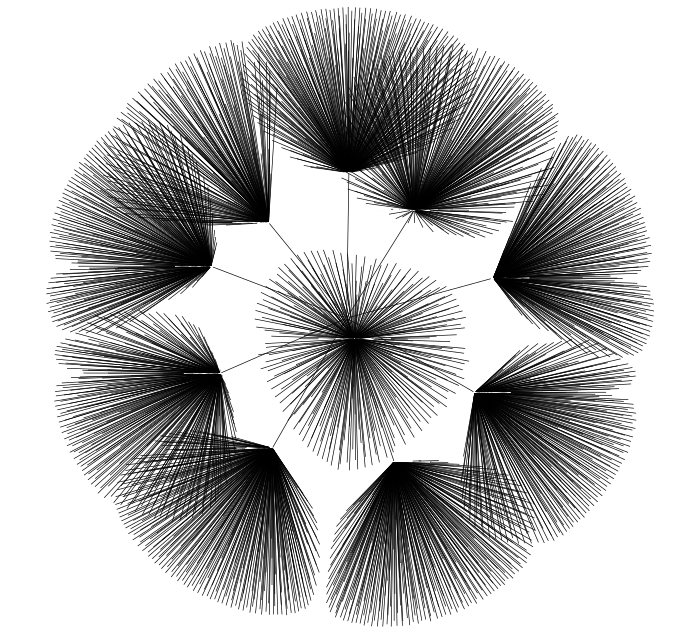
\includegraphics[width=0.5\textwidth,center]{neato-btree.png}
        }
    \end{center}
\end{frame}

\begin{frame}[fragile]{}
    \frametitle{}

    \begin{itemize}[label={\MVRightarrow}]
        \item <+-> Comer D. (1979). The Ubiquitous B-Tree. \\
            Computing Surveys, 11 (2).
        \item <+-> Graefe G. (2011). Modern B-Tree Techniques. \\
            Foundations and Trends in Databases.
    \end{itemize}
\end{frame}

\begin{frame}[fragile]{}
    \frametitle{}

    \begin{itemize}[label={\MVRightarrow}]
        \item RUM conjecture
        \item B-Tree internals
        \begin{itemize}[label={}]
            \item \footnotesize{Key normalization}
            \item \footnotesize{Prefix/Suffix truncation}
            %\item SB-Tree
        \end{itemize}
        \item B-Tree as a component
        \begin{itemize}[label={}]
            \item \footnotesize{Hybrid index}
            \item \footnotesize{Bw-Tree}
            \item \footnotesize{Partitioned B-Tree}
        \end{itemize}
        \item Learned Indexes
        \item Everything else
    \end{itemize}
\end{frame}
\note{
    small sub points
}

\section{RUM conjecture}

\begin{frame}
    \frametitle{}
    \begin{center}

    \only<1>
    {
        \begin{tikzpicture}[]
            \node [rum-node] (memory) at ( 3, 0) {Mem};
            \node [rum-node] (write) at (-3, 0) {Write};
            \node [rum-node] (read) at ( 0, 3) {Read};
            \draw (read) -- (write) -- (memory) -- (read);
            \begin{scope}[on background layer]
                \fill [gray, opacity=0.2]
                    (read.center) --
                    (write.center) --
                    (memory.center) -- cycle;
            \end{scope}
        \end{tikzpicture}
    }

    \only<2>
    {
        \begin{tikzpicture}[]
            \node [rum-node, fill=greenGood] (memory) at ( 3, 0) {Mem};
            \node [rum-node, fill=redBad] (write) at (-3, 0) {Write};
            \node [rum-node, fill=greenGood] (read) at ( 0, 3) {Read};
            \draw (read) -- (write) -- (memory) -- (read);
            \begin{scope}[on background layer]
                \fill [gray, opacity=0.2]
                    (read.center) --
                    (write.center) --
                    (memory.center) -- cycle;
            \end{scope}
        \end{tikzpicture}
    }

    \end{center}
\end{frame}

\section{B-Tree internals}

\begin{frame}[fragile]{}
    \frametitle{}

    \begin{center}
    \textbf{B-Tree $\,\to\,$ B$^+$Tree}
    \vspace{1cm}

    \begin{overprint}[12cm]
        \onslide<1>
        \begin{tikzpicture}[]
            \btreenode{1}{}{btree-hide}{}{}
            \btreenode{2}{below=1cm of node1.south}{btree-hide}{}{}
            \btreenode{3}{below=1cm of node1.south west, xshift=-3cm}{btree-hide}{}{}
            \btreenode{4}{below=1cm of node1.south east, xshift=3cm}{btree-hide}{}{}

            \draw[->, btree-line] (pointer11.south) -- (pointer12.north);
            \draw[->, btree-line] (pointer21.south)
                .. controls ([yshift=-1cm] pointer21) and ([yshift=1cm] pointer14) ..
                (pointer14.north);
            \draw[->, btree-line] (pointer31.south)
                .. controls ([yshift=-1cm] pointer31) and ([yshift=1cm] pointer13) ..
                (pointer13.north);

            \coordinate[right=0.5cm of sep34.east] (link-sep34);
            \draw[btree-hide] ([yshift=0.1cm]sep34.east) -- ([yshift=0.1cm]link-sep34.west);
            \coordinate[left=0.5cm of sep43.west] (link-sep43);
            \draw[btree-hide] ([yshift=0.1cm]sep43.west) -- ([yshift=0.1cm]link-sep43.east);
        \end{tikzpicture}

        \onslide<2>
        \begin{tikzpicture}[]
            \btreenode{1}{}{btree-hide}{btree-branch}{}
            \btreenode{2}{below=1cm of node1.south}{btree-hide}{btree-leaf}{}
            \btreenode{3}{below=1cm of node1.south west, xshift=-3cm}{btree-hide}{btree-leaf}{}
            \btreenode{4}{below=1cm of node1.south east, xshift=3cm}{btree-hide}{btree-leaf}{}

            \draw[->, btree-line] (pointer11.south) -- (pointer12.north);
            \draw[->, btree-line] (pointer21.south)
                .. controls ([yshift=-1cm] pointer21) and ([yshift=1cm] pointer14) ..
                (pointer14.north);
            \draw[->, btree-line] (pointer31.south)
            .. controls ([yshift=-1cm] pointer31) and ([yshift=1cm] pointer13) ..
            (pointer13.north);

            \coordinate[right=0.5cm of sep34.east] (link-sep34);
            \draw[btree-hide] ([yshift=0.1cm]sep34.east) -- ([yshift=0.1cm]link-sep34.west);
            \coordinate[left=0.5cm of sep43.west] (link-sep43);
            \draw[btree-hide] ([yshift=0.1cm]sep43.west) -- ([yshift=0.1cm]link-sep43.east);
        \end{tikzpicture}

        \onslide<3>
        \begin{tikzpicture}[]
            \btreenode{1}{}{}{btree-branch}{}
            \btreenode{2}{below=1cm of node1.south}
                {}{btree-leaf}{show-pointers}
            \btreenode{3}{below=1cm of node1.south west, xshift=-3cm}
                {}{btree-leaf}{show-pointers}
            \btreenode{4}{below=1cm of node1.south east, xshift=3cm}
                {}{btree-leaf}{show-pointers}

            \draw[->, btree-line] (pointer11.south) -- (pointer12.north);
            \draw[->, btree-line] (pointer21.south)
                .. controls ([yshift=-1cm] pointer21) and ([yshift=1cm] pointer14) ..
                (pointer14.north);
            \draw[->, btree-line] (pointer31.south)
                .. controls ([yshift=-1cm] pointer31) and ([yshift=1cm] pointer13) ..
                (pointer13.north);

            \coordinate[right=0.5cm of sep34.east] (link-sep34);
            \draw[btree-hide] ([yshift=0.1cm]sep34.east) -- ([yshift=0.1cm]link-sep34.west);
            \coordinate[left=0.5cm of sep43.west] (link-sep43);
            \draw[btree-hide] ([yshift=0.1cm]sep43.west) -- ([yshift=0.1cm]link-sep43.east);
        \end{tikzpicture}

        \onslide<4>
        \begin{tikzpicture}[]
            \btreenode{1}{}{}{btree-branch}{}
            \btreenode{2}{below=1cm of node1.south}
                {}{btree-leaf}{show-pointers}
            \btreenode{3}{below=1cm of node1.south west, xshift=-3cm}
                {}{btree-leaf}{show-pointers}
            \btreenode{4}{below=1cm of node1.south east, xshift=3cm}
                {}{btree-leaf}{show-pointers}

            \draw[->, btree-line] (pointer11.south) -- (pointer12.north);
            \draw[->, btree-line] (pointer21.south)
                .. controls ([yshift=-1cm] pointer21) and ([yshift=1cm] pointer14) ..
                (pointer14.north);
            \draw[->, btree-line] (pointer31.south)
                .. controls ([yshift=-1cm] pointer31) and ([yshift=1cm] pointer13) ..
                (pointer13.north);

            \draw[->, btree-line] ([yshift=0.1cm]sep33.east) -- ([yshift=0.1cm]sep42.west);
            \draw[->, btree-line] ([yshift=0.1cm]sep32.east) -- ([yshift=0.1cm]sep44.west);
            \coordinate[right=0.5cm of sep34.east] (link-sep34);
            \draw[->, btree-line] ([yshift=0.1cm]sep34.east) -- ([yshift=0.1cm]link-sep34.west);
            \coordinate[left=0.5cm of sep43.west] (link-sep43);
            \draw[btree-hide] ([yshift=0.1cm]sep43.west) -- ([yshift=0.1cm]link-sep43.east);
        \end{tikzpicture}

        \onslide<5>
        \begin{tikzpicture}[]
            \btreenode{1}{}{}{btree-branch}{}
            \btreenode{2}{below=1cm of node1.south}
                {}{btree-leaf}{show-pointers}
            \btreenode{3}{below=1cm of node1.south west, xshift=-3cm}
                {}{btree-leaf}{show-pointers}
            \btreenode{4}{below=1cm of node1.south east, xshift=3cm}
                {}{btree-leaf}{show-pointers}

            \draw[->, btree-line] (pointer11.south) -- (pointer12.north);
            \draw[->, btree-line] (pointer21.south)
                .. controls ([yshift=-1cm] pointer21) and ([yshift=1cm] pointer14) ..
                (pointer14.north);
            \draw[->, btree-line] (pointer31.south)
                .. controls ([yshift=-1cm] pointer31) and ([yshift=1cm] pointer13) ..
                (pointer13.north);

            \draw[->, btree-line] ([yshift=0.1cm]sep33.east) -- ([yshift=0.1cm]sep42.west);
            \draw[->, btree-line] ([yshift=0.1cm]sep32.east) -- ([yshift=0.1cm]sep44.west);
            \draw[<-, btree-line] ([yshift=-0.1cm]sep33.east) -- ([yshift=-0.1cm]sep42.west);
            \draw[<-, btree-line] ([yshift=-0.1cm]sep32.east) -- ([yshift=-0.1cm]sep44.west);
            \coordinate[right=0.5cm of sep34.east] (link-sep34);
            \draw[->, btree-line] ([yshift=0.1cm]sep34.east) -- ([yshift=0.1cm]link-sep34.west);
            \coordinate[left=0.5cm of sep43.west] (link-sep43);
            \draw[->, btree-line] ([yshift=0.1cm]sep43.west) -- ([yshift=0.1cm]link-sep43.east);
        \end{tikzpicture}

        \onslide<6>
        \begin{tikzpicture}[]
            \btreenode{1}{}{}{btree-branch}{}
            \btreenode{2}{below=1cm of node1.south}
                {}{btree-leaf}{show-pointers}
            \btreenode{3}{below=1cm of node1.south west, xshift=-3cm}
                {}{btree-leaf}{show-pointers}
            \btreenode{4}{below=1cm of node1.south east, xshift=3cm}
                {}{btree-leaf}{show-pointers}

            \draw[->, btree-line, color=red, line width=2pt] (pointer11.south) -- (pointer12.north);
            \draw[->, btree-line] (pointer21.south)
                .. controls ([yshift=-1cm] pointer21) and ([yshift=1cm] pointer14) ..
                (pointer14.north);
            \draw[->, btree-line] (pointer31.south)
                .. controls ([yshift=-1cm] pointer31) and ([yshift=1cm] pointer13)
                .. (pointer13.north);

            \path
              node[btree-path, below=-0.505 of pointer11.west] (path-pointer1) {}
              node[btree-path, below=-0.505 of pointer32.west] (path-pointer2) {};

            \draw[->, btree-line, color=red, line width=2pt]
                (pointer32.south) -- (heap-pointer32.north);

            \draw[->, btree-line] ([yshift=0.1cm]sep33.east) -- ([yshift=0.1cm]sep42.west);
            \draw[->, btree-line] ([yshift=0.1cm]sep32.east) -- ([yshift=0.1cm]sep44.west);
            \draw[<-, btree-line] ([yshift=-0.1cm]sep33.east) -- ([yshift=-0.1cm]sep42.west);
            \draw[<-, btree-line] ([yshift=-0.1cm]sep32.east) -- ([yshift=-0.1cm]sep44.west);
            \coordinate[right=0.5cm of sep34.east] (link-sep34);
            \draw[->, btree-line] ([yshift=0.1cm]sep34.east) -- ([yshift=0.1cm]link-sep34.west);
            \coordinate[left=0.5cm of sep43.west] (link-sep43);
            \draw[->, btree-line] ([yshift=0.1cm]sep43.west) -- ([yshift=0.1cm]link-sep43.east);
        \end{tikzpicture}
    \end{overprint}

    \linespread{0.5}
    \vspace{0.5cm}
    \color{black}\fontsize{6pt}{0}\selectfont
        Lehman P., Yao S. (1981). Efficient Locking for Concurrent Operations on B-Trees. \\
        ACM Transactions on Database Systems.
    \linespread{1.5}
    \end{center}

\end{frame}
\note{
    Postgres uses variation of B-link Tree, seems like MySQL innodb uses
    regular B+ Tree.

    WiredTiger uses parent pointers.
}

\fontsize{17pt}{18}\selectfont
\begin{frame}[fragile]{}
    \frametitle{}

    \begin{center}
    \textbf{Page split}
    \vspace{1cm}

    \begin{overprint}[8cm]
        \onslide<1>
        \begin{tikzpicture}[]
            \btreenodewithitems{1}{5}{2}{}{btree-branch}
            \btreenodewithitems{2}{5}{4}{below=1cm of key11, xshift=-2cm}{btree-leaf}
            \draw[->, btree-line] (node1.south)
                .. controls ([yshift=-1cm] node1) and ([yshift=1.2cm] node2) ..
                (node2.north);
        \end{tikzpicture}

        \onslide<2>
        \begin{tikzpicture}[]
            \btreenodewithitems{1}{5}{2}{}{btree-branch}
            \btreenodewithitems{2}{5}{4}{below=1cm of key11, xshift=-2cm}{btree-leaf}
            \draw[->, btree-line] (node1.south)
                .. controls ([yshift=-1cm] node1) and ([yshift=1.2cm] node2) ..
                (node2.north);

            \node[btree-key, below=1cm of key23] (new-key) {};
            \draw[->, btree-line] (new-key.east)
                .. controls ([xshift=1cm] new-key) and (key24) ..
                (key24.center);
        \end{tikzpicture}

        \onslide<3>
        \begin{tikzpicture}[]
            \btreenodewithitems{1}{5}{2}{}{btree-branch}
            \btreenodewithitems{2}{5}{3}{below=1cm of key11, xshift=-2cm}{btree-leaf}
            \btreenodewithitems{3}{5}{3}{below=1cm of key11, xshift=2cm}{btree-leaf}
            \draw[->, btree-line] (node1.south)
                .. controls ([yshift=-1cm] node1) and ([yshift=1.2cm] node2) ..
                (node2.north);
            \draw[->, btree-line] (node1.south)
                .. controls ([yshift=-1cm] node1) and ([yshift=1.2cm] node3) ..
                (node3.north);
        \end{tikzpicture}

        \onslide<4>
        \begin{tikzpicture}[]
            \btreenodewithitems{1}{5}{2}{}{btree-branch}
            \btreenodewithitems{2}{5}{3}{below=1cm of key11, xshift=-2cm}{btree-leaf}
            \btreenodewithitems{3}{5}{3}{below=1cm of key11, xshift=2cm}{btree-leaf}
            \draw[->, btree-line] (node1.south)
                .. controls ([yshift=-1cm] node1) and ([yshift=1.2cm] node2) ..
                (node2.north);
            \draw[->, btree-line] (node1.south)
                .. controls ([yshift=-1cm] node1) and ([yshift=1.2cm] node3) ..
                (node3.north);

            \node[btree-key, below=-0.5cm of key13.center] (promoted) {};
            \draw[->, btree-line] (key31.west)
                .. controls ([xshift=-1cm] key31) and (promoted) ..
                (promoted.center);
        \end{tikzpicture}

    \end{overprint}
    \end{center}

\end{frame}
\note{
    B*-Tree rebalances between neighbors, e.g. as in SQLite.
}

\begin{frame}[fragile]{}
    \frametitle{}

    \begin{center}
    \textbf{Page merge}
    %\vspace{1cm}
    \end{center}

    \begin{flushleft}
        \begin{displayquote}
            "By adding periodic rebuilding of the tree, we obtain a data
            structure that is theoreticaly superior to standard B-trees in many
            ways. Our results suggest that rebalancing on deletion no only
            unnecessary but may be harmful."
        \end{displayquote}
        \footnotesize{Sen S., Tarjan R. E. (2009). Deletion without rebalancing
            in multiway search trees ACM Transactions on Database Systems}
    \end{flushleft}

\end{frame}
\note{
    Postgres deletes via marking a tuple as dead, and then vacuuming either a
    table of a single page.
}

\begin{frame}[fragile]{}
    \frametitle{}

    \begin{center}
    \textbf{Key normalization}
    \vspace{1cm}

    \begin{tabular}{cccl}
        1 & "Dirk" & "Bart" &
            \colorbox{BurntOrange}{1}
            \colorbox{SpringGreen}{0..01}
            \colorbox{BurntOrange}{1}
            \colorbox{SpringGreen}{11..00}
            \colorbox{Gray!40}{$\emptyset$}
            \colorbox{BurntOrange}{1}
            \colorbox{SpringGreen}{10..10}
            \colorbox{Gray!40}{$\emptyset$} \\
        2 & "Todd" & Null &
            \colorbox{BurntOrange}{1}
            \colorbox{SpringGreen}{0..10}
            \colorbox{BurntOrange}{1}
            \colorbox{SpringGreen}{01..00}
            \colorbox{Gray!40}{$\emptyset$}
            \colorbox{BurntOrange}{0} \\
        Null & "" & Null &
            \colorbox{BurntOrange}{0}
            \colorbox{BurntOrange}{1}
            \colorbox{Gray!40}{$\emptyset$}
            \colorbox{BurntOrange}{0} \\
    \end{tabular}

    \linespread{0.5}
    \vspace{0.5cm}
    \color{black}\fontsize{6pt}{0}\selectfont
        Singleton, R. C. (1969). An efficient algorithm for sorting with minimal storage. \\
        Communications of the ACM.
    \linespread{1.5}

    \end{center}
\end{frame}
\note{
    https://wiki.postgresql.org/wiki/Key_normalization

    Should be not used for leaves, since normalization looses the information.
    Other option is too store both normalized and original key values.
}

\begin{frame}[fragile]{}
    \frametitle{}

    \begin{center}
    \textbf{Prefix truncation}
    \vspace{1cm}

    \begin{overprint}[8cm]
        \onslide<1>
        \begin{tabular}{lll}
            & & \\
            & Smith Jack & 01-02-2019 \\
            & Smith Jane & 02-03-2019 \\
            & Smith James & 03-04-2019 \\
        \end{tabular}

        \onslide<2>
        \begin{tabular}{lll}
            & & \\
            & \colorbox{BurntOrange}{Smith Ja}ck & 01-02-2019 \\
            & \colorbox{BurntOrange}{Smith Ja}ne & 02-03-2019 \\
            & \colorbox{BurntOrange}{Smith Ja}mes & 03-04-2019 \\
        \end{tabular}

        \onslide<3>
        \begin{tabular}{lll}
            \colorbox{BurntOrange}{Smith Ja} & & \\
            & ck & 01-02-2019 \\
            & ne & 02-03-2019 \\
            & mes & 03-04-2019 \\
        \end{tabular}

        \onslide<4>
        \begin{center}
        \begin{tikzpicture}[]
            \btreenodewithitems{1}{8}{5}{}{btree-leaf}
            \coordinate[below=1cm of key11] (start1);
            \coordinate[below=1cm of high-key1] (start2);
            \draw[->, btree-line, line width=1.5pt, shorten >= 2mm] (start1) -- (key11);
            \draw[->, btree-line, line width=1.5pt, shorten >= 2mm] (start2) -- (high-key1);
        \end{tikzpicture}
        \end{center}

        %\onslide<5>
        %\begin{center}
        %\begin{tikzpicture}[]
            %\btreenodewithitems{1}{8}{5}{}{btree-leaf}
            %\foreach \i in {1,...,4}
            %{
                %\coordinate[below=1cm of key1\i] (start\i);
                %\draw[->, btree-line, line width=1.5pt, shorten >= 2mm] (start\i) -- (key1\i);
            %}
        %\end{tikzpicture}
        %\end{center}

    \end{overprint}

    \end{center}
\end{frame}
\note{
    BerkleyDB, https://web.stanford.edu/class/cs276a/projects/docs/berkeleydb/api_c/db_set_bt_prefix.html

    TODO: mark shared parts of keys in both situations
}

\begin{frame}[fragile]{}
    \frametitle{}

    \begin{center}
    \textbf{Dynamic prefix truncation}
    \vspace{1cm}

    \begin{overprint}[8cm]
        \onslide<1>
        \begin{center}
        \begin{tikzpicture}[]
            \btreenodewithitems{1}{8}{5}{}{btree-leaf}
            \node[btree-key, below=1cm of key13.center] (compared) {};
        \end{tikzpicture}
        \end{center}

        \onslide<2>
        \begin{center}
        \begin{tikzpicture}[]
            \btreenodewithitems{1}{8}{5}{}{btree-leaf}
            \node[btree-key, below=1cm of key13.center] (compared) {};

            \node[btree-key-prefix, below=1cm of key13.center] (compared-prefix) {};
            \node[btree-key-prefix, below=-0.5cm of high-key1.center] (compared-high-key-prefix) {};
            \node[btree-key-prefix, below=-0.5cm of key11.center] (compared-first-key-prefix) {};
        \end{tikzpicture}
        \end{center}

        \onslide<3>
        \begin{center}
        \begin{tikzpicture}[]
            \btreenodewithitems{1}{8}{5}{}{btree-leaf}
            \node[btree-key, below=1cm of key13.center] (compared) {};

            \node[btree-key-prefix, below=1cm of key13.center] (compared-prefix) {};
            \node[btree-key-prefix, below=-0.5cm of high-key1.center] (compared-high-key-prefix) {};
            \node[btree-key-prefix, below=-0.5cm of key11.center] (compared-first-key-prefix) {};

            \node[btree-key-compare, below=-0.1cm of compared.center] (compare-key) {};
            \foreach \i in {1,...,4}
            {
                \node[btree-key-compare, below=-0.1cm of key1\i.center] (compare-\i) {};
            }
        \end{tikzpicture}
        \end{center}

    \end{overprint}

    \end{center}
\end{frame}

\begin{frame}[fragile]{}
    \frametitle{}

    \begin{center}
    \textbf{Suffix truncation}
    \vspace{1cm}

    \begin{overprint}[8cm]
        \onslide<1>
        \begin{tabular}{lll}
            & Cohen Richard & 02-02-2019 \\
            & Johnson David & 04-02-2019 \\
            & Miller Kevin & 01-02-2019 \\
            & Miller Mary & 02-03-2019 \\
            & Miller Steven & 03-04-2019 \\
            & Smith Susan & 01-02-2019 \\
        \end{tabular}

        \onslide<2>
        \begin{tabular}{lll}
            & Cohen Richard & 02-02-2019 \\
            & Johnson David & 04-02-2019 \\
            & Miller Kevin & 01-02-2019 \\
            \hline
            & \colorbox{BurntOrange}{Miller M}ary & 02-03-2019 \\
            & Miller Steven & 03-04-2019 \\
            & Smith Susan & 01-02-2019 \\
        \end{tabular}

        \onslide<3>
        \begin{tabular}{lll}
            & Cohen Richard & 02-02-2019 \\
            \hline
            & \colorbox{BurntOrange}{J}ohnson David & 04-02-2019 \\
            & Miller Kevin & 01-02-2019 \\
            & Miller Mary & 02-03-2019 \\
            & Miller Steven & 03-04-2019 \\
            & Smith Susan & 01-02-2019 \\
        \end{tabular}

    \end{overprint}

    \linespread{0.5}
    \vspace{0.5cm}
    \color{black}\fontsize{6pt}{0}\selectfont
        Bayer, R., Unterauer, K. (1977). Prefix B-trees. \\
        ACM Transactions on Database Systems.
    \linespread{1.5}

    \end{center}
\end{frame}
\note{
    Not a normalized version, but whole column version is in PG12.
}

\fontsize{17pt}{18}\selectfont
\begin{frame}[fragile]{}
    \frametitle{}

    \begin{center}
    \textbf{Page split}
    \vspace{1cm}

    \begin{overprint}[6cm]
        \onslide<1>
        \begin{tikzpicture}[]
            \btreenodewithitems{1}{5}{2}{}{btree-branch}
            \btreenodewithitems{2}{5}{3}{below=1cm of key11, xshift=-2cm}{btree-leaf}
            \btreenodewithitems{3}{5}{3}{below=1cm of key11, xshift=2cm}{btree-leaf}
            \draw[->, btree-line] (node1.south)
                .. controls ([yshift=-1cm] node1) and ([yshift=1.2cm] node2) ..
                (node2.north);
            \draw[->, btree-line] (node1.south)
                .. controls ([yshift=-1cm] node1) and ([yshift=1.2cm] node3) ..
                (node3.north);

            \node[btree-key, below=-0.5cm of key13.center] (promoted) {};
            \draw[->, btree-line, color=red, line width=0.5mm] (key31.west)
                .. controls ([xshift=-1cm] key31) and (promoted) ..
                (promoted.center);
        \end{tikzpicture}

    \end{overprint}
    \end{center}

\end{frame}

\begin{frame}[fragile]{}
    \frametitle{}

    \begin{center}
    \textbf{Indirection vector}
    \vspace{1cm}

    \begin{overprint}[8cm]
        \onslide<1>
        \begin{center}
        \begin{tikzpicture}[]
            \btreenodewithindirection{1}{5}{5}{minimum height=1.5cm}{btree-leaf}

            \foreach \i/ \shift in {1/0.35cm,2/0.11cm,3/-0.07cm,4/-0.3cm} {
                \draw[->, btree-line] ([yshift=\shift]indirection-key1\i.east) -- ([yshift=\shift]key1\i.center);
            }
          \linespread{0.5}
          \node[cpu-cache-hide, below=1cm of indirection-key12.east]
              (cpu-cache) {\footnotesize{CPU\\Cache}};

          \coordinate[above=2cm of cpu-cache.north east] (cpu-cache-top-left);
          \coordinate[above=2cm of cpu-cache.north west] (cpu-cache-top-right);
          \draw[draw=none] ([xshift=-0.2cm]cpu-cache.north east) -- ([xshift=-0.2cm]cpu-cache-top-left);
          \draw[draw=none] ([xshift=0.2cm]cpu-cache.north west) -- ([xshift=0.2cm]cpu-cache-top-right);

          \linespread{1.5}

        \end{tikzpicture}
        \end{center}

        \onslide<2>
        \begin{center}
        \begin{tikzpicture}[]
            \btreenodewithindirection{1}{5}{5}{minimum height=1.5cm}{btree-leaf}

            \foreach \i/ \shift/ \letter in {1/-0.6cm/a,2/-0.4cm/b,3/-0.2cm/c,4/-0.0cm/d} {
              \node[draw=none, below=\shift of indirection-key1\i.center]
                (normalized-indirection-key1\i) {\tiny{\textbf{\letter}}};
            }

            \foreach \i/ \shift in {1/0.35cm,2/0.11cm,3/-0.07cm,4/-0.3cm} {
                \draw[->, btree-line] ([yshift=\shift]indirection-key1\i.east) -- ([yshift=\shift]key1\i.center);
            }

          \linespread{0.5}
          \node[cpu-cache-hide, below=1cm of indirection-key12.east]
              (cpu-cache) {\footnotesize{CPU\\Cache}};

          \coordinate[above=2cm of cpu-cache.north east] (cpu-cache-top-left);
          \coordinate[above=2cm of cpu-cache.north west] (cpu-cache-top-right);
          \draw[draw=none] ([xshift=-0.2cm]cpu-cache.north east) -- ([xshift=-0.2cm]cpu-cache-top-left);
          \draw[draw=none] ([xshift=0.2cm]cpu-cache.north west) -- ([xshift=0.2cm]cpu-cache-top-right);

          \linespread{1.5}

        \end{tikzpicture}
        \end{center}

        \onslide<3>
        \begin{center}
        \begin{tikzpicture}[]
            \btreenodewithindirection{1}{5}{5}{minimum height=1.5cm}{btree-leaf}

            \foreach \i/ \shift/ \letter in {1/-0.6cm/a,2/-0.4cm/b,3/-0.2cm/c,4/-0.0cm/d} {
              \node[draw=none, below=\shift of indirection-key1\i.center]
                (normalized-indirection-key1\i) {\tiny{\textbf{\letter}}};
            }

            \foreach \i/ \shift in {1/0.35cm,2/0.11cm,3/-0.07cm,4/-0.3cm} {
                \draw[->, btree-line] ([yshift=\shift]indirection-key1\i.east) -- ([yshift=\shift]key1\i.center);
            }

          \linespread{0.5}
          \node[cpu-cache, below=1.5cm of indirection-key12.east]
              (cpu-cache) {\footnotesize{CPU\\Cache}};

          \coordinate[above=2.5cm of cpu-cache.north east] (cpu-cache-top-left);
          \coordinate[above=2.5cm of cpu-cache.north west] (cpu-cache-top-right);
          \draw[dashed] ([xshift=-0.2cm]cpu-cache.north east) -- ([xshift=-0.2cm]cpu-cache-top-left);
          \draw[dashed] ([xshift=0.2cm]cpu-cache.north west) -- ([xshift=0.2cm]cpu-cache-top-right);

          \linespread{1.5}

        \end{tikzpicture}
        \end{center}
    \end{overprint}

    \linespread{0.5}
    \vspace{0.5cm}
    \color{black}\fontsize{6pt}{0}\selectfont
        Graefe G., Larson P. (2001). B-tree indexes and CPU caches. \\
        International Conference on Data Engineering.
    \linespread{1.5}

    \end{center}
\end{frame}
\note{
    Another interesting approach is partial value on a page and the rest is on
    extended pages (MySQL InnoDB, SQLite).
}

%\begin{frame}[fragile]{}
    %\frametitle{}

    %\begin{center}
    %\textbf{SB-tree}
    %\vspace{1cm}

    %\begin{overprint}[15cm]
        %\onslide<1>
        %\begin{tikzpicture}[]
            %\btreenode{1}{}{btree-hide}{btree-branch}{}
            %\btreenode{2}{right=2cm of node1.east}{btree-hide}{btree-branch}{}
            %\node[btree-hide, right=2cm of node2.east, minimum width=0.5cm] (node2-extra) {};

            %\btreenode{3}{below=1cm of node1.south west, xshift=-0.5cm}{btree-hide}{btree-leaf}{}
            %\btreenode{4}{below=1cm of node1.south east, xshift=0.5cm}{btree-hide}{btree-leaf}{}
            %\btreenode{5}{right=2cm of node4.east}{btree-hide}{btree-leaf}{}
            %\node[btree-hide, right=2cm of node5.east, minimum width=0.5cm] (node5-extra) {};

            %\draw[->, btree-line] (pointer21.south)
                %.. controls ([yshift=-1cm] pointer21) and ([yshift=1cm] pointer14) ..
                %(pointer14.north);
            %\draw[->, btree-line] (pointer31.south)
                %.. controls ([yshift=-1cm] pointer31) and ([yshift=1cm] pointer13) ..
                %(pointer13.north);

            %\node[box, inner sep=0.2cm,
                %fit=(node1)(node2)(node2-extra)
            %] (extent-1) {};

            %\node[box, inner sep=0.2cm,
                %fit=(node3)(node4)(node5)(node5-extra)
            %] (extent-2) {};
        %\end{tikzpicture}

        %\onslide<2>
        %\begin{tikzpicture}[]
            %\btreenode{1}{}{btree-hide}{btree-branch}{}
            %\btreenode{2}{right=2cm of node1.east}{btree-hide}{btree-branch}{}
            %\node[btree-hide, right=2cm of node2.east, minimum width=0.5cm] (node2-extra) {};

            %\btreenode{3}{below=1cm of node1.south west, xshift=-0.5cm}{btree-hide}{btree-leaf}{}
            %\btreenode{4}{below=1cm of node1.south east, xshift=0.5cm}{btree-hide}{btree-leaf}{}
            %\btreenode{5}{right=2cm of node4.east}{btree-hide}{btree-leaf}{}
            %\node[btree-hide, right=2cm of node5.east, minimum width=0.5cm] (node5-extra) {};

            %\draw[->, btree-line] (pointer21.south)
                %.. controls ([yshift=-1cm] pointer21) and ([yshift=1cm] pointer14) ..
                %(pointer14.north);
            %\draw[->, btree-line] (pointer31.south)
                %.. controls ([yshift=-1cm] pointer31) and ([yshift=1cm] pointer13) ..
                %(pointer13.north);

            %\node[box, inner sep=0.2cm,
                %fit=(node1)(node2)(node2-extra)
            %] (extent-1) {};

            %\node[box, inner sep=0.2cm,
                %fit=(node3)(node4)(node5)(node5-extra)
            %] (extent-2) {};

            %\draw[->, btree-line] (node5.center)
                %.. controls ([yshift=-1cm] node5) and ([yshift=-1cm,xshift=-1cm] node5-extra) ..
                %([xshift=-1cm]node5-extra.center);
        %\end{tikzpicture}
    %\end{overprint}

    %\linespread{0.5}
    %\vspace{0.5cm}
    %\color{black}\fontsize{6pt}{0}\selectfont
        %O’Neil P. E. (1992). The SB-tree: An index-sequential structure for high performance sequential access. \\
        %Acta Informatica.
    %\linespread{1.5}

    %\end{center}
%\end{frame}
%\note{
    %OrientDB uses SB-Tree, but are they the same?
%}

%\begin{frame}[fragile]{}
    %\frametitle{}

    %\begin{center}
    %\textbf{Multidimentional Access Method}
    %\vspace{1cm}

    %\begin{overprint}[8cm]
        %\onslide<1>
        %\begin{tikzpicture}[]
            %\basicbtree{show-connections}
            %\node[below=0.2 of node5] {\footnotesize{1,a}};
            %\node[below=1.8 of node2] {\footnotesize{...}};
            %\node[below=0.2 of node6] {\footnotesize{1,z}};

            %\node[below=0.2 of node7] {\footnotesize{2,a}};
            %\node[below=1.8 of node3] {\footnotesize{...}};
            %\node[below=0.2 of node8] {\footnotesize{2,z}};

            %\node[below=0.2 of node9] {\footnotesize{3,a}};
            %\node[below=1.8 of node4] {\footnotesize{...}};
            %\node[below=0.2 of node10] {\footnotesize{3,z}};
        %\end{tikzpicture}

        %\onslide<2>
        %\begin{tikzpicture}[]
            %\basicbtree{show-connections}
            %\node[below=0.2 of node5] {\footnotesize{1,a}};
            %\node[below=1.8 of node2] {\footnotesize{...}};
            %\node[below=0.2 of node6] {\footnotesize{1,z}};

            %\node[below=0.2 of node7] {\footnotesize{2,a}};
            %\node[below=1.8 of node3] {\footnotesize{...}};
            %\node[below=0.2 of node8] {\footnotesize{2,z}};

            %\node[below=0.2 of node9] {\footnotesize{3,a}};
            %\node[below=1.8 of node4] {\footnotesize{...}};
            %\node[below=0.2 of node10] {\footnotesize{3,z}};

            %\draw[selected-path] (node1.center) -- (node2.center) -- (node5.center);
        %\end{tikzpicture}

        %\onslide<3>
        %\begin{tikzpicture}[]
            %\basicbtree{show-connections}
            %\node[below=0.2 of node5] {\footnotesize{1,a}};
            %\node[below=1.8 of node2] {\footnotesize{...}};
            %\node[below=0.2 of node6] {\footnotesize{1,z}};

            %\node[below=0.2 of node7] {\footnotesize{2,a}};
            %\node[below=1.8 of node3] {\footnotesize{...}};
            %\node[below=0.2 of node8] {\footnotesize{2,z}};

            %\node[below=0.2 of node9] {\footnotesize{3,a}};
            %\node[below=1.8 of node4] {\footnotesize{...}};
            %\node[below=0.2 of node10] {\footnotesize{3,z}};

            %\draw[selected-path] (node1.center) -- (node3.center) -- (node7.center);
        %\end{tikzpicture}

        %\onslide<4>
        %\begin{tikzpicture}[]
            %\basicbtree{show-connections}
            %\node[below=0.2 of node5] {\footnotesize{1,a}};
            %\node[below=1.8 of node2] {\footnotesize{...}};
            %\node[below=0.2 of node6] {\footnotesize{1,z}};

            %\node[below=0.2 of node7] {\footnotesize{2,a}};
            %\node[below=1.8 of node3] {\footnotesize{...}};
            %\node[below=0.2 of node8] {\footnotesize{2,z}};

            %\node[below=0.2 of node9] {\footnotesize{3,a}};
            %\node[below=1.8 of node4] {\footnotesize{...}};
            %\node[below=0.2 of node10] {\footnotesize{3,z}};

            %\draw[selected-path] (node1.center) -- (node4.center) -- (node9.center);
        %\end{tikzpicture}
    %\end{overprint}

    %\linespread{0.5}
    %\color{black}\fontsize{6pt}{0}\selectfont
        %Leslie, H., Jain, R., Birdsall, D., Yaghmai, H. (1995). Efficient search of multi-dimensional b-trees. VLDB.
    %\linespread{1.5}

    %\end{center}
%\end{frame}
%\note{
    %For not complete search keys, if a dimension is under-specified, its
    %possible values must be enumerated.
%}

\begin{frame}[fragile]{}
    \frametitle{}

    \begin{center}
    \begin{overprint}[8cm]
        \onslide<1>
        \begin{tikzpicture}[]
            \node [rum-node] (memory) at ( 3, 0) {Mem};
            \node [rum-node] (write) at (-3, 0) {Write};
            \node [rum-node] (read) at ( 0, 3) {Read};
            \draw (read) -- (write) -- (memory) -- (read);
            \begin{scope}[on background layer]
                \fill [gray, opacity=0.2]
                    (read.center) --
                    (write.center) --
                    (memory.center) -- cycle;
            \end{scope}

            \coordinate[below=0.5 of read] (btree-pointer);
            \coordinate[right=2 of read] (btree-angle);
            \node[above=0.5 of btree-angle, draw=none, color=white] (btree) {B-Tree};
        \end{tikzpicture}

        \onslide<2>
        \begin{tikzpicture}[]
            \node [rum-node, fill=redBad] (memory) at ( 3, 0) {Mem};
            \node [rum-node, fill=redBad] (write) at (-3, 0) {Write};
            \node [rum-node, fill=greenGood] (read) at ( 0, 3) {Read};
            \draw (read) -- (write) -- (memory) -- (read);
            \begin{scope}[on background layer]
                \fill [gray, opacity=0.2]
                    (read.center) --
                    (write.center) --
                    (memory.center) -- cycle;
            \end{scope}

            \coordinate[below=0.5 of read] (btree-pointer);
            \coordinate[right=2 of read] (btree-angle);
            \node[above=0.5 of btree-angle, draw=none] (btree) {B-Tree};
            \draw[->, line width=2pt] (btree)
                .. controls ([yshift=-2cm] btree) and (btree-pointer) ..
                (btree-pointer);
        \end{tikzpicture}
    \end{overprint}
    \end{center}
\end{frame}

\begin{frame}[fragile]{}
    \frametitle{}

    \begin{center}
        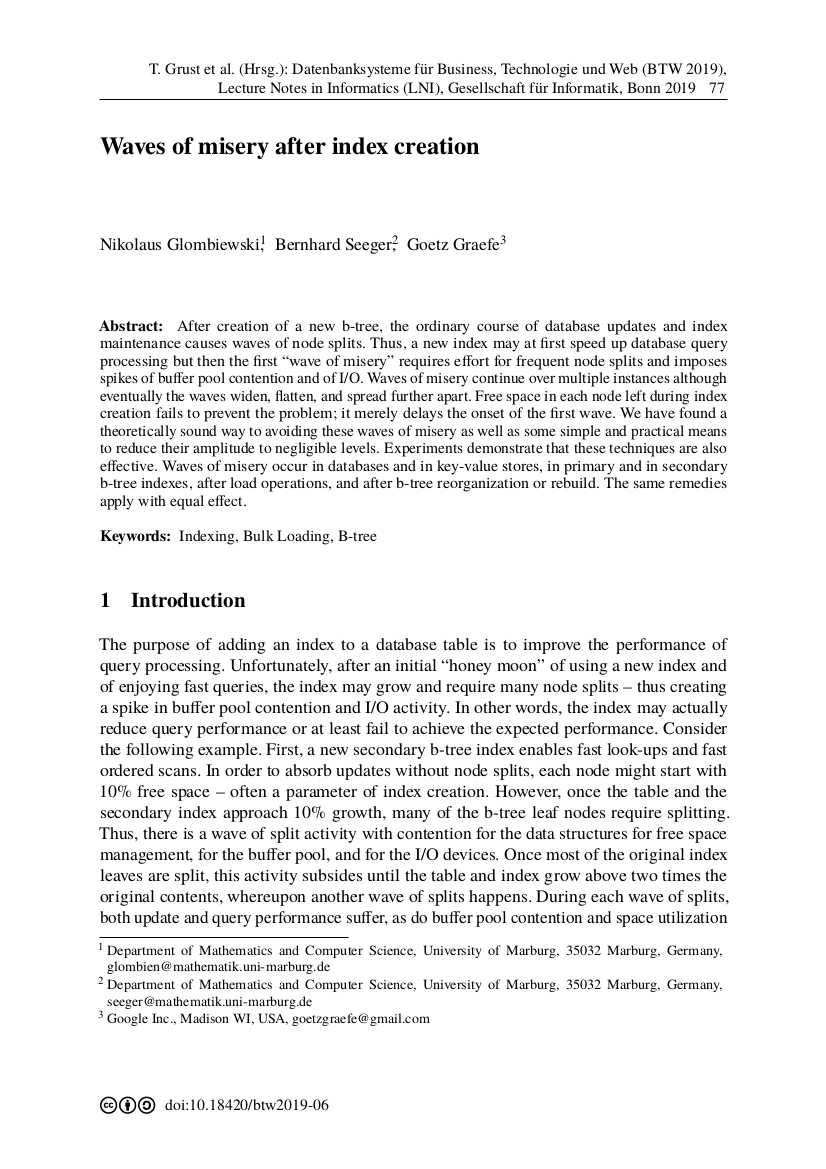
\includegraphics[width=0.65\textwidth,center]{waves.png}
    \end{center}
\end{frame}

\section{B-Tree as a component}

\begin{frame}[fragile]{}
    \frametitle{}

    \def\arraystretch{1.5}
    \begin{overprint}[8cm]
        \onslide<1>
        \begin{tabular}{cccc}
            \colorbox{white}{B-Tree} & \colorbox{white}{B$^{+}$-Tree} & \colorbox{white}{B$_{link}$-Tree} & \colorbox{white}{DPTree} \\
            wB$^{+}$-Tree & NV-Tree & FPTree & FASTFAIR \\
            HiKV & Masstree & Skip List & ART \\
            WORT & CDDS-Tree & \colorbox{white}{Bw-Tree} & HOT \\
            KISS-Tree & VAST-Tree & FAST & HV-Tree \\
            UB-Tree & LHAM & \colorbox{white}{PBT} & \colorbox{white}{Hybrid B$^{+}$-Tree}
        \end{tabular}

        \onslide<2>
        \begin{tabular}{cccc}
            \colorbox{red!20}{B-Tree} & \colorbox{red!20}{B$^{+}$-Tree} & \colorbox{red!20}{B$_{link}$-Tree} & DPTree \\
            wB$^{+}$-Tree & NV-Tree & FPTree & FASTFAIR \\
            HiKV & Masstree & Skip List & ART \\
            WORT & CDDS-Tree & \colorbox{white}{Bw-Tree} & HOT \\
            KISS-Tree & VAST-Tree & FAST & HV-Tree \\
            UB-Tree & LHAM & \colorbox{white}{PBT} & \colorbox{white}{Hybrid B$^{+}$-Tree}
        \end{tabular}

        \onslide<3>
        \begin{tabular}{cccc}
            \colorbox{red!20}{B-Tree} & \colorbox{red!20}{B$^{+}$-Tree} & \colorbox{red!20}{B$_{link}$-Tree} & \colorbox{red!20}{DPTree} \\
            wB$^{+}$-Tree & NV-Tree & FPTree & FASTFAIR \\
            HiKV & Masstree & Skip List & ART \\
            WORT & CDDS-Tree & \colorbox{red!20}{Bw-Tree} & HOT \\
            KISS-Tree & VAST-Tree & FAST & HV-Tree \\
            UB-Tree & LHAM & \colorbox{red!20}{PBT} & \colorbox{red!20}{Hybrid B$^{+}$-Tree}
        \end{tabular}

    \end{overprint}

\end{frame}

\begin{frame}[fragile]{}
    \frametitle{}

    \begin{center}
    \textbf{Partitioned B-tree}
    \vspace{1cm}

    \begin{overprint}[8cm]
        \onslide<1>
        \begin{tikzpicture}[]
            \node[btree-node] (node1) {};

            \node[btree-node, below=0.5cm of node1.south west, xshift=-2.5cm] (node2) {};
            \node[btree-node, below=0.5cm of node1.south] (node3) {};
            \node[btree-node, below=0.5cm of node1.south east, xshift=2.5cm] (node4) {};

            \node[btree-node, below=0.5cm of node2.south west, xshift=-0.2cm] (node5) {};
            \node[btree-node, below=0.5cm of node2.south east, xshift=0.2cm] (node6) {};

            \node[btree-node, below=0.5cm of node3.south west, xshift=-0.2cm] (node7) {};
            \node[btree-node, below=0.5cm of node3.south east, xshift=0.2cm] (node8) {};

            \node[btree-node, below=0.5cm of node4.south west, xshift=-0.2cm] (node9) {};
            \node[btree-node, below=0.5cm of node4.south east, xshift=0.2cm] (node10) {};

            \draw[->, btree-line] (node1) -- (node2);
            \draw[->, btree-line] (node1) -- (node3);
            \draw[->, btree-line] (node1) -- (node4);

            \draw[->, btree-line] (node2) -- (node5);
            \draw[->, btree-line] (node2) -- (node6);

            \draw[->, btree-line] (node3) -- (node7);
            \draw[->, btree-line] (node3) -- (node8);

            \draw[->, btree-line] (node4) -- (node9);
            \draw[->, btree-line] (node4) -- (node10);
        \end{tikzpicture}

        \onslide<2>
        \begin{tikzpicture}[]
            \node[btree-node] (node1) {};

            \node[btree-node, below=0.5cm of node1.south west, xshift=-2.5cm] (node2) {};
            \node[btree-node, below=0.5cm of node1.south] (node3) {};
            \node[btree-partition1, below=0.5cm of node1.south east, xshift=2.5cm] (node4) {};

            \node[btree-node, below=0.5cm of node2.south west, xshift=-0.2cm] (node5) {};
            \node[btree-node, below=0.5cm of node2.south east, xshift=0.2cm] (node6) {};

            \node[btree-node, below=0.5cm of node3.south west, xshift=-0.2cm] (node7) {};
            \node[btree-node, below=0.5cm of node3.south east, xshift=0.2cm] (node8) {};

            \node[btree-partition1, below=0.5cm of node4.south west, xshift=-0.2cm] (node9) {};
            \node[btree-partition1, below=0.5cm of node4.south east, xshift=0.2cm] (node10) {};

            \draw[->, btree-line] (node1) -- (node2);
            \draw[->, btree-line] (node1) -- (node3);
            \draw[->, btree-line] (node1) -- (node4);

            \draw[->, btree-line] (node2) -- (node5);
            \draw[->, btree-line] (node2) -- (node6);

            \draw[->, btree-line] (node3) -- (node7);
            \draw[->, btree-line] (node3) -- (node8);

            \draw[->, btree-line] (node4) -- (node9);
            \draw[->, btree-line] (node4) -- (node10);
        \end{tikzpicture}

        \onslide<3>
        \begin{tikzpicture}[]
            \node[btree-node] (node1) {};

            \node[btree-partition1, below=0.5cm of node1.south west, xshift=-2.5cm] (node2) {};
            \node[btree-partition2, below=0.5cm of node1.south] (node3) {};
            \node[btree-partition3, below=0.5cm of node1.south east, xshift=2.5cm] (node4) {};

            \node[btree-partition1, below=0.5cm of node2.south west, xshift=-0.2cm] (node5) {};
            \node[btree-partition1, below=0.5cm of node2.south east, xshift=0.2cm] (node6) {};

            \node[btree-partition2, below=0.5cm of node3.south west, xshift=-0.2cm] (node7) {};
            \node[btree-partition2, below=0.5cm of node3.south east, xshift=0.2cm] (node8) {};

            \node[btree-partition3, below=0.5cm of node4.south west, xshift=-0.2cm] (node9) {};
            \node[btree-partition3, below=0.5cm of node4.south east, xshift=0.2cm] (node10) {};

            \draw[->, btree-line] (node1) -- (node2);
            \draw[->, btree-line] (node1) -- (node3);
            \draw[->, btree-line] (node1) -- (node4);

            \draw[->, btree-line] (node2) -- (node5);
            \draw[->, btree-line] (node2) -- (node6);

            \draw[->, btree-line] (node3) -- (node7);
            \draw[->, btree-line] (node3) -- (node8);

            \draw[->, btree-line] (node4) -- (node9);
            \draw[->, btree-line] (node4) -- (node10);

            \node[arrow-pointer, below=3cm of node2.center, rotate=90, yshift=0.2cm] {};
            \node[arrow-pointer, below=3cm of node3.center, rotate=90, yshift=0.2cm] {};
            \node[arrow-pointer, below=3cm of node4.center, rotate=90, yshift=0.2cm] {};
            \node[below=3cm of node3.center, minimum height=1cm] {};

        \end{tikzpicture}
        \linespread{0.5}
        \color{black}\fontsize{6pt}{0}\selectfont
            Graefe G. (2003). Sorting and indexing with partitioned B-Trees. \\
            Classless Inter Domain Routing
        \linespread{1.5}

        \onslide<4>
        \begin{tikzpicture}[]
            \node[btree-node] (node1) {};

            \node[btree-partition1, below=0.5cm of node1.south west, xshift=-2.5cm] (node2) {};
            \node[btree-partition2, below=0.5cm of node1.south] (node3) {};
            \node[btree-partition3, below=0.5cm of node1.south east, xshift=2.5cm] (node4) {};

            \node[btree-partition1, below=0.5cm of node2.south west, xshift=-0.2cm] (node5) {};
            \node[btree-partition1, below=0.5cm of node2.south east, xshift=0.2cm] (node6) {};

            \node[btree-partition2, below=0.5cm of node3.south west, xshift=-0.2cm] (node7) {};
            \node[btree-partition2, below=0.5cm of node3.south east, xshift=0.2cm] (node8) {};

            \node[btree-partition3, below=0.5cm of node4.south west, xshift=-0.2cm] (node9) {};
            \node[btree-partition3, below=0.5cm of node4.south east, xshift=0.2cm] (node10) {};

            \draw[->, btree-line] (node1) -- (node2);
            \draw[->, btree-line] (node1) -- (node3);
            \draw[->, btree-line] (node1) -- (node4);

            \draw[->, btree-line] (node2) -- (node5);
            \draw[->, btree-line] (node2) -- (node6);

            \draw[->, btree-line] (node3) -- (node7);
            \draw[->, btree-line] (node3) -- (node8);

            \draw[->, btree-line] (node4) -- (node9);
            \draw[->, btree-line] (node4) -- (node10);

            \draw[->, btree-line] ([yshift=-2cm]node2.center)
                .. controls ([yshift=-3cm] node2) and ([yshift=-3cm] node3) ..
                ([yshift=-2cm]node3.center);
            \draw[->, btree-line] ([yshift=-2cm]node4.center)
                .. controls ([yshift=-3cm] node4) and ([yshift=-3cm] node3) ..
                ([yshift=-2cm]node3.center);
            \node[below=3cm of node3.center, minimum height=1cm] {};

        \end{tikzpicture}
        \linespread{0.5}
        \color{black}\fontsize{6pt}{0}\selectfont
            Graefe G. (2003). Sorting and indexing with partitioned B-Trees. \\
            Classless Inter Domain Routing
        \linespread{1.5}

        \onslide<5>
        \begin{tikzpicture}[]
            \node[btree-node] (node1) {};

            \node[btree-node, below=0.5cm of node1.south west, xshift=-2.5cm] (node2) {};
            \node[btree-node, below=0.5cm of node1.south] (node3) {};
            \node[btree-partition1, below=0.5cm of node1.south east, xshift=2.5cm] (node4) {};

            \node[btree-node, below=0.5cm of node2.south west, xshift=-0.2cm] (node5) {};
            \node[btree-node, below=0.5cm of node2.south east, xshift=0.2cm] (node6) {};

            \node[btree-node, below=0.5cm of node3.south west, xshift=-0.2cm] (node7) {};
            \node[btree-node, below=0.5cm of node3.south east, xshift=0.2cm] (node8) {};

            \node[btree-partition1, below=0.5cm of node4.south west, xshift=-0.2cm] (node9) {};
            \node[btree-partition1, below=0.5cm of node4.south east, xshift=0.2cm] (node10) {};

            \draw[->, btree-line] (node1) -- (node2);
            \draw[->, btree-line] (node1) -- (node3);
            \draw[->, btree-line] (node1) -- (node4);

            \draw[->, btree-line] (node2) -- (node5);
            \draw[->, btree-line] (node2) -- (node6);

            \draw[->, btree-line] (node3) -- (node7);
            \draw[->, btree-line] (node3) -- (node8);

            \draw[->, btree-line] (node4) -- (node9);
            \draw[->, btree-line] (node4) -- (node10);

            \node[arrow-pointer, right=2cm of node9.center, rotate=-135, xshift=-2.7cm, yshift=-1cm] {};
            \node[box, fit=(node4)(node9)(node10)] {};
            \node[below=3cm of node3.center, minimum height=1cm] {};

        \end{tikzpicture}
        \linespread{0.5}
        \color{black}\fontsize{6pt}{0}\selectfont
            Riegger C., Vincon T., Petrov I. (2017). Write-optimized indexing with partitioned b-trees. \\
            Proceedings of the 19th International Conference on Information Integration and Web-based Applications \& Services
        \linespread{1.5}

        \onslide<6>
        \begin{tikzpicture}[]
            \node[btree-node] (node1) {};

            \node[btree-node, below=0.5cm of node1.south west, xshift=-2.5cm] (node2) {};
            \node[btree-node, below=0.5cm of node1.south] (node3) {};
            \node[btree-partition1, below=0.5cm of node1.south east, xshift=2.5cm] (node4) {};

            \node[btree-node, below=0.5cm of node2.south west, xshift=-0.2cm] (node5) {};
            \node[btree-node, below=0.5cm of node2.south east, xshift=0.2cm] (node6) {};

            \node[btree-node, below=0.5cm of node3.south west, xshift=-0.2cm] (node7) {};
            \node[btree-node, below=0.5cm of node3.south east, xshift=0.2cm] (node8) {};

            \node[btree-partition1, below=0.5cm of node4.south west, xshift=-0.2cm] (node9) {};
            \node[btree-partition1, below=0.5cm of node4.south east, xshift=0.2cm] (node10) {};

            \draw[->, btree-line] (node1) -- (node2);
            \draw[->, btree-line] (node1) -- (node3);
            \draw[->, btree-line] (node1) -- (node4);

            \draw[->, btree-line] (node2) -- (node5);
            \draw[->, btree-line] (node2) -- (node6);

            \draw[->, btree-line] (node3) -- (node7);
            \draw[->, btree-line] (node3) -- (node8);

            \draw[->, btree-line] (node4) -- (node9);
            \draw[->, btree-line] (node4) -- (node10);

            \node[arrow-pointer, right=2cm of node9.center, rotate=-135, xshift=-2.7cm, yshift=-1cm] {};
            \node[box, fit=(node4)(node9)(node10)] {};
            \node[below=3cm of node3.center, minimum height=1cm] {};

            \draw[->, btree-line] ([yshift=-2cm]node4.center)
                .. controls ([yshift=-3cm] node4) and ([yshift=-3cm] node3) ..
                ([yshift=-2cm]node3.center);
            \draw[->, btree-line] ([yshift=-2cm]node4.center)
                .. controls ([yshift=-4cm] node4) and ([yshift=-4cm] node2) ..
                ([yshift=-2cm]node2.center);

        \end{tikzpicture}
        \linespread{0.5}
        \color{black}\fontsize{6pt}{0}\selectfont
            Riegger C., Vincon T., Petrov I. (2017). Write-optimized indexing with partitioned b-trees. \\
            Proceedings of the 19th International Conference on Information Integration and Web-based Applications \& Services
        \linespread{1.5}

    \end{overprint}

    \end{center}
\end{frame}
\note{
    For faster index creation, via pushing all merge runs into btree into
    different partitions.
}

\begin{frame}[fragile]{}
    \frametitle{}

    \begin{center}
    \textbf{Hybrid indexes}
    \vspace{1cm}

    \begin{overprint}[12cm]
        \onslide<1>
        \begin{tikzpicture}[]
            \smallbtree{1}{2.5}{}{}{}{green-box}
            \node[draw, color=white, left=4cm of node11, minimum width=1.2cm,
                  minimum height=0.4cm, yshift=-0.6cm] (node21) {};
            \node[bloom-filter, color=white, above=0.5cm of node21] (bloom) {};
            \node[arrow-pointer, left=0.5cm of node21.west, color=white] {\footnotesize{Insert}};
        \end{tikzpicture}

        \onslide<2>
        \begin{tikzpicture}[]
            \smallbtree{1}{2.5}{}{}{}{green-box}
            \smallbtree{2}{1}{left=4cm of node11, yshift=-0.6cm}{color=blue!20}{color=blue!20}{blue-box}
            \node[bloom-filter, color=white, above=0.5cm of node21] (bloom) {};
            \node[arrow-pointer, left=0.5cm of nodebox2.west, color=white] {\footnotesize{Insert}};
        \end{tikzpicture}

        \onslide<3>
        \begin{tikzpicture}[]
            \smallbtree{1}{2.5}{}{}{}{green-box}
            \smallbtree{2}{1}{left=4cm of node11, yshift=-0.6cm}{}{}{blue-box}
            \node[bloom-filter, color=white, above=0.5cm of node21] (bloom) {};
            \node[arrow-pointer, left=0.5cm of nodebox2.west, color=white] {\footnotesize{Insert}};
        \end{tikzpicture}

        \onslide<4>
        \begin{tikzpicture}[]
            \smallbtree{1}{2.5}{}{}{}{green-box}
            \smallbtree{2}{1}{left=4cm of node11, yshift=-0.6cm}{}{}{blue-box}
            \node[bloom-filter, above=0.5cm of node21, fill=redBad] (bloom) {};
            \node[arrow-pointer, left=0.5cm of nodebox2.west, color=white] {\footnotesize{Insert}};
        \end{tikzpicture}

        \onslide<5>
        \begin{tikzpicture}[]
            \smallbtree{1}{2.5}{}{}{}{green-box}
            \smallbtree{2}{1}{left=4cm of node11, yshift=-0.6cm}{}{}{blue-box}
            \node[bloom-filter, above=0.5cm of node21, fill=redBad] (bloom) {};
            \node[arrow-pointer, left=0.5cm of nodebox2.west, color=white] (inserts) {\footnotesize{Insert}};
            \node[arrow-pointer, above=1.2cm of inserts] {\footnotesize{Read}};

            \draw[->, btree-line] (bloom.south) -- (nodebox2.north);
            \draw[->, btree-line] (bloom.east) -| (nodebox1.north);
        \end{tikzpicture}

        \onslide<6>
        \begin{tikzpicture}[]
            \smallbtree{1}{2.5}{}{}{}{green-box}
            \smallbtree{2}{1}{left=4cm of node11, yshift=-0.6cm}{}{}{blue-box}
            \node[bloom-filter, above=0.5cm of node21, fill=redBad] (bloom) {};
            \node[arrow-pointer, left=0.5cm of nodebox2.west] (inserts) {\footnotesize{Insert}};
            \node[arrow-pointer, above=1.2cm of inserts] {\footnotesize{Read}};

            \draw[->, btree-line] ([yshift=-0.2cm]nodebox2.south)
                .. controls ([yshift=-2.5cm] nodebox2) and ([yshift=-2.5cm] nodebox1) ..
                ([yshift=-0.2cm]nodebox1.south);

            \draw[->, btree-line] (bloom.south) -- (nodebox2.north);
            \draw[->, btree-line] (bloom.east) -| (nodebox1.north);
        \end{tikzpicture}
    \end{overprint}

    \linespread{0.5}
    \vspace{0.5cm}
    \color{black}\fontsize{6pt}{0}\selectfont
        Zhang H., Andersen D. G., Pavlo A., Kaminsky M., Ma L., Shen R. (2016). \\
        Reducing the Storage Overhead of Main-Memory OLTP Databases with Hybrid
        Indexes. \\
        Proceedings of the 2016 International Conference on Management of Data
        (SIGMOD ’16)
    \linespread{1.5}

    \end{center}
\end{frame}
\note{
    Designed for B-Tree, Masstree, Skip List, ART
}

\begin{frame}[fragile]{}
    \frametitle{}

    \begin{center}
    \textbf{Bw-Tree}
    \vspace{1cm}

    \begin{overprint}[12cm]
        \onslide<1>
        \begin{tikzpicture}[]
            \basicbtree{show-connections}
        \end{tikzpicture}

        \onslide<2>
        \begin{tikzpicture}[]
            \basicbtree{}
            \coordinate[right=0.25cm of node1.center] (link-anchor1);
            \node[below=-0.05cm of link-anchor1] (link1) {\footnotesize{1}};

            \coordinate[right=0.25cm of node3.center] (link-anchor2);
            \node[below=-0.05cm of link-anchor2] (link2) {\footnotesize{2}};

            \draw[->, btree-line, color=white] (node1) -- (node2);
            \draw[->, btree-line, color=white] (node1) -- (node3);
            \draw[->, btree-line, dashed] (node1) -- (node4);

            \draw[->, btree-line, color=white] (node2) -- (node5);
            \draw[->, btree-line, color=white] (node2) -- (node6);

            \draw[->, btree-line, color=white] (node3) -- (node7);
            \draw[->, btree-line, dashed] (node3) -- (node8);

            \draw[->, btree-line, color=white] (node4) -- (node9);
            \draw[->, btree-line, color=white] (node4) -- (node10);

            \path
                node[draw, right=5cm of node1.east, minimum width=1.2cm] (header1) {\textbf{\normalsize{ID}}}
                node[draw, right=0 of header1, minimum width=1.2cm] (header2) {\textbf{\normalsize{PTR}}}
                    node[draw, below=0 of header1, minimum width=1.2cm] (row11) {\normalsize{1}}
                    node[draw, right=0 of row11, minimum width=1.2cm] (row12) {\normalsize{0x...}}
                    node[draw, below=0 of row11, minimum width=1.2cm] (row21) {\normalsize{2}}
                    node[draw, right=0 of row21, minimum width=1.2cm] (row22) {\normalsize{0x...}}
                    node[behind path, fit=(header1)(header2)(row11)(row12)(row21)(row22)] (mapping) {};

            \draw[->, btree-line] (row11.west)
            .. controls ([xshift=-1cm] row11) and ([yshift=2cm] node4) ..
            (node4.center);

            \draw[->, btree-line] (row21.west)
            .. controls ([xshift=-2cm] row21) and ([xshift=2cm] node8) ..
            (node8.center);
        \end{tikzpicture}

        \onslide<3>
        \begin{tikzpicture}[]
            \path
                node[draw, right=5cm of node1.east, minimum width=1.2cm] (header1) {\textbf{\normalsize{ID}}}
                node[draw, right=0 of header1, minimum width=1.2cm] (header2) {\textbf{\normalsize{PTR}}}
                    node[draw, below=0 of header1, minimum width=1.2cm] (row11) {\normalsize{1}}
                    node[draw, right=0 of row11, minimum width=1.2cm] (row12) {\normalsize{0x...}}
                    node[draw, below=0 of row11, minimum width=1.2cm] (row21) {\normalsize{2}}
                    node[draw, right=0 of row21, minimum width=1.2cm] (row22) {\normalsize{0x...}}
                    node[behind path, fit=(header1)(header2)(row11)(row12)(row21)(row22)] (mapping) {};

            \node[bw-delta, right=4cm of header2, color=white] (delta) {$\Delta$};
            \node[bw-page, below=0.5cm of delta] (page) {Page};
            \draw[->, btree-line] (row22)
                .. controls ([yshift=-2cm] row22) and ([yshift=-2cm] page) ..
            (page);
        \end{tikzpicture}

        \onslide<4>
        \begin{tikzpicture}[]
            \path
                node[draw, right=5cm of node1.east, minimum width=1.2cm] (header1) {\textbf{\normalsize{ID}}}
                node[draw, right=0 of header1, minimum width=1.2cm] (header2) {\textbf{\normalsize{PTR}}}
                    node[draw, below=0 of header1, minimum width=1.2cm] (row11) {\normalsize{1}}
                    node[draw, right=0 of row11, minimum width=1.2cm] (row12) {\normalsize{0x...}}
                    node[draw, below=0 of row11, minimum width=1.2cm] (row21) {\normalsize{2}}
                    node[draw, right=0 of row21, minimum width=1.2cm] (row22) {\normalsize{0x...}}
                    node[behind path, fit=(header1)(header2)(row11)(row12)(row21)(row22)] (mapping) {};

            \node[bw-delta, right=4cm of header2] (delta) {$\Delta$};
            \node[bw-page, below=0.5cm of delta] (page) {Page};
            \draw[->, btree-line] (delta) -- (page);
            \draw[->, btree-line] (row22)
                .. controls ([yshift=-2cm] row22) and ([yshift=-2cm] page) ..
            (page);
        \end{tikzpicture}

        \onslide<5>
        \begin{tikzpicture}[]
            \path
                node[draw, right=5cm of node1.east, minimum width=1.2cm] (header1) {\textbf{\normalsize{ID}}}
                node[draw, right=0 of header1, minimum width=1.2cm] (header2) {\textbf{\normalsize{PTR}}}
                    node[draw, below=0 of header1, minimum width=1.2cm] (row11) {\normalsize{1}}
                    node[draw, right=0 of row11, minimum width=1.2cm] (row12) {\normalsize{0x...}}
                    node[draw, below=0 of row11, minimum width=1.2cm] (row21) {\normalsize{2}}
                    node[draw, right=0 of row21, minimum width=1.2cm] (row22) {\normalsize{0x...}}
                    node[behind path, fit=(header1)(header2)(row11)(row12)(row21)(row22)] (mapping) {};

            \node[bw-delta, right=4cm of header2] (delta) {$\Delta$};
            \node[bw-page, below=0.5cm of delta] (page) {Page};
            \draw[->, btree-line] (delta) -- (page);
            \draw[->, btree-line, dashed, color=gray] (row22)
                .. controls ([yshift=-2cm] row22) and ([yshift=-2cm] page) ..
                node[midway, above, color=gray] {\footnotesize{CAS}} (page);
            \draw[->, btree-line] (row22)
                .. controls ([xshift=2cm] row22) and ([xshift=-2cm] delta) ..
            (delta);
        \end{tikzpicture}

        \onslide<6>
        \begin{tikzpicture}[]
            \path
                node[draw, right=5cm of node1.east, minimum width=1.2cm] (header1) {\textbf{\normalsize{ID}}}
                node[draw, right=0 of header1, minimum width=1.2cm] (header2) {\textbf{\normalsize{PTR}}}
                    node[draw, below=0 of header1, minimum width=1.2cm] (row11) {\normalsize{1}}
                    node[draw, right=0 of row11, minimum width=1.2cm] (row12) {\normalsize{0x...}}
                    node[draw, below=0 of row11, minimum width=1.2cm] (row21) {\normalsize{2}}
                    node[draw, right=0 of row21, minimum width=1.2cm] (row22) {\normalsize{0x...}}
                    node[behind path, fit=(header1)(header2)(row11)(row12)(row21)(row22)] (mapping) {};

            \node[bw-delta, right=5cm of header2] (delta1) {$\Delta_1$};
            \node[bw-delta, left=0.5cm of delta1] (delta2) {$\Delta_2$};
            \node[bw-delta, left=0.5cm of delta2] (delta3) {$\Delta_3$};
            \node[bw-page, below=0.5cm of delta2] (page) {Page};
            \node[behind path, fit=(delta1)(delta2)(delta3)(page), rounded corners, color=white] (merged) {};
            \draw[->, btree-line] (delta1) -- (delta2) -- (delta3) -- (page);
            \draw[->, btree-line] (row22)
                .. controls ([xshift=2cm] row22) and ([xshift=-2cm] delta3) ..
            (delta3);
        \end{tikzpicture}

        \onslide<7>
        \begin{tikzpicture}[]
            \path
                node[draw, right=5cm of node1.east, minimum width=1.2cm] (header1) {\textbf{\normalsize{ID}}}
                node[draw, right=0 of header1, minimum width=1.2cm] (header2) {\textbf{\normalsize{PTR}}}
                    node[draw, below=0 of header1, minimum width=1.2cm] (row11) {\normalsize{1}}
                    node[draw, right=0 of row11, minimum width=1.2cm] (row12) {\normalsize{0x...}}
                    node[draw, below=0 of row11, minimum width=1.2cm] (row21) {\normalsize{2}}
                    node[draw, right=0 of row21, minimum width=1.2cm] (row22) {\normalsize{0x...}}
                    node[behind path, fit=(header1)(header2)(row11)(row12)(row21)(row22)] (mapping) {};

            \path
                node[bw-delta, right=5cm of header2] (delta1) {$\Delta_1$}
                node[bw-delta, left=0.5cm of delta1] (delta2) {$\Delta_2$}
                node[bw-delta, left=0.5cm of delta2] (delta3) {$\Delta_3$}
                node[bw-page, below=0.5cm of delta2] (page) {Page}
                node[behind path, fill=gray!20, fit=(delta1)(delta2)(delta3)(page), rounded corners] (merged) {};
            \draw[->, btree-line] (delta1) -- (delta2) -- (delta3) -- (page);
            \draw[->, btree-line] (row22)
                .. controls ([xshift=2cm] row22) and ([xshift=-2cm] delta3) ..
            (delta3);

            \node[bw-page, below=1cm of page] (merged-page) {Merged Page};
            \draw[->, btree-line] (merged.south) -- (merged-page);
        \end{tikzpicture}

        \onslide<8>
        \begin{tikzpicture}[]
            \path
                node[draw, right=5cm of node1.east, minimum width=1.2cm] (header1) {\textbf{\normalsize{ID}}}
                node[draw, right=0 of header1, minimum width=1.2cm] (header2) {\textbf{\normalsize{PTR}}}
                    node[draw, below=0 of header1, minimum width=1.2cm] (row11) {\normalsize{1}}
                    node[draw, right=0 of row11, minimum width=1.2cm] (row12) {\normalsize{0x...}}
                    node[draw, below=0 of row11, minimum width=1.2cm] (row21) {\normalsize{2}}
                    node[draw, right=0 of row21, minimum width=1.2cm] (row22) {\normalsize{0x...}}
                    node[behind path, fit=(header1)(header2)(row11)(row12)(row21)(row22)] (mapping) {};

            \path
                node[bw-delta, right=5cm of header2] (delta1) {$\Delta_1$}
                node[bw-delta, left=0.5cm of delta1] (delta2) {$\Delta_2$}
                node[bw-delta, left=0.5cm of delta2] (delta3) {$\Delta_3$}
                node[bw-page, below=0.5cm of delta2] (page) {Page}
                node[behind path, fill=gray!20, fit=(delta1)(delta2)(delta3)(page), rounded corners] (merged) {};
            \draw[->, btree-line] (delta1) -- (delta2) -- (delta3) -- (page);
            \draw[->, btree-line, color=gray, dashed] (row22)
                .. controls ([xshift=2cm] row22) and ([xshift=-2cm] delta3) ..
            node[midway, above, color=gray] {\footnotesize{CAS}} (delta3);

            \node[bw-page, below=1cm of page, rounded corners] (merged-page) {Merged Page};
            \draw[->, btree-line] (merged.south) -- (merged-page);
            \draw[->, btree-line] (row22)
                .. controls ([xshift=2cm] row22) and ([xshift=-3cm] merged-page) ..
            (merged-page.west);
        \end{tikzpicture}

    \end{overprint}

    \linespread{0.5}
    \vspace{0.5cm}
    \color{black}\fontsize{6pt}{0}\selectfont
        Levandoski J., Lomet D., Sengupta S. (2012). The Bw-Tree: A B-tree for
        New Hardware Platforms. \\
        International Conference on Data Engineering.
    \linespread{1.5}

    \end{center}
\end{frame}
\note{
    Requires also "split", "index", "remove node", "merge", "flush" deltas
    MSFT Hekaton, Sled db - Bw-Tree
}

\begin{frame}[fragile]{}
    \frametitle{}

    \begin{center}
    \textbf{DPTree}
    \vspace{1cm}

    \begin{overprint}[14cm]
        \onslide<1>
        \begin{tikzpicture}[]
            \basicbtree{show-connections}

            \coordinate[above=0.25cm of node5] (left-point);
            \coordinate[above=0.25cm of node10] (right-point);

            \draw[color=white, opacity=0] ([xshift=-5cm]left-point) -- ([xshift=1cm]right-point);

            \smallbtree{1}{1.5}{left=6cm of node1}{color=white}{color=white}{color=white}

            \coordinate[left=1.2cm of nodebox1.south west] (inserts-start);
            \coordinate[left=1.2cm of nodebox1.north west] (reads-start);
            \node[arrow-pointer, above=0.2cm of inserts-start, color=white] (inserts) {\footnotesize{Insert}};
            \node[arrow-pointer, below=0.2cm of reads-start, color=white] (reads) {\footnotesize{Read}};
        \end{tikzpicture}

        \onslide<2>
        \begin{tikzpicture}[]
            \basicbtree{show-connections}

            \coordinate[above=0.25cm of node5] (left-point);
            \coordinate[above=0.25cm of node10] (right-point);

            \draw[color=white, opacity=0] ([xshift=-5cm]left-point) -- ([xshift=1cm]right-point);

            \smallbtree{1}{1.5}{left=6cm of node1}{}{}{blue-box}

            \coordinate[left=1.2cm of nodebox1.south west] (inserts-start);
            \coordinate[left=1.2cm of nodebox1.north west] (reads-start);
            \node[arrow-pointer, above=0.2cm of inserts-start, color=white] (inserts) {\footnotesize{Insert}};
            \node[arrow-pointer, below=0.2cm of reads-start, color=white] (reads) {\footnotesize{Read}};
        \end{tikzpicture}

        \onslide<3>
        \begin{tikzpicture}[]
            \basicbtree{show-connections}
            \basicleafconnection{active}

            \coordinate[above=0.25cm of node5] (left-point);
            \coordinate[above=0.25cm of node10] (right-point);

            \draw[dashed] ([xshift=-5cm]left-point) -- ([xshift=1cm]right-point);

            \smallbtree{1}{1.5}{left=6cm of node1}{}{}{blue-box}

            \coordinate[left=1.2cm of nodebox1.south west] (inserts-start);
            \coordinate[left=1.2cm of nodebox1.north west] (reads-start);
            \node[arrow-pointer, above=0.2cm of inserts-start, color=white] (inserts) {\footnotesize{Insert}};
            \node[arrow-pointer, below=0.2cm of reads-start, color=white] (reads) {\footnotesize{Read}};
        \end{tikzpicture}

        \onslide<4>
        \begin{tikzpicture}[]
            \basicbtree{show-fade-connections}
            \basicleafconnection{}

            \coordinate[above=0.25cm of node5] (left-point);
            \coordinate[above=0.25cm of node10] (right-point);

            \draw[dashed] ([xshift=-5cm]left-point) -- ([xshift=1cm]right-point);

            \smallbtree{1}{1.5}{left=6cm of node1}{}{}{blue-box}
            \node[dp-tree-log, below=1.5cm of nodebox1.south] (log2) {};
            \node[dp-tree-log, right=0.5cm of log2] (log3) {};
            \node[dp-tree-log, left=0.5cm of log2] (log1) {};
            \draw[->, btree-line] (nodebox1.south) -- (log3);
            \draw[->, btree-line] (log1) -- (log2) -- (log3);

            \coordinate[left=1.2cm of nodebox1.south west] (inserts-start);
            \coordinate[left=1.2cm of nodebox1.north west] (reads-start);
            \node[arrow-pointer, above=0.2cm of inserts-start] (inserts) {\footnotesize{Insert}};
            \node[arrow-pointer, below=0.2cm of reads-start] (reads) {\footnotesize{Read}};

            \node[arrow-pointer, left=2cm of node1] {\footnotesize{Read}};
            \node[arrow-pointer, right=0.2cm of nodebox1.south east, rotate=-45, fill=white] {\footnotesize{Merge}};
        \end{tikzpicture}

    \end{overprint}

    \linespread{0.5}
    \vspace{0.5cm}
    \color{black}\fontsize{6pt}{0}\selectfont
         Zhou Xinjing, Shou Lidan, Chen Ke, Hu Wei, Chen Gang. (2019). DPTree:
         differential indexing for persistent memory. \\
         Proceedings of the VLDB Endowment.
    \linespread{1.5}

    \end{center}
\end{frame}

\section{Learned Indexes}

\begin{frame}[fragile]{}
    \frametitle{}

    \begin{center}
    \textbf{Learned Indexes}
    \vspace{1.0cm}

    \begin{overprint}[3cm]
        \onslide<1>
        \begin{tikzpicture}[]
            \smallbtree{1}{2.5}{}{}{}{green-box}
            \node[dp-tree-log, below=1.5cm of nodebox1.south] (log2) {};
            \node[dp-tree-log, right=0.5cm of log2] (log3) {};
            \node[dp-tree-log, left=0.5cm of log2] (log1) {};
            \draw[->, btree-line] (nodebox1.south) -- (log3);
            \draw[->, btree-line] (nodebox1.south) -- (log2);
            \draw[->, btree-line] (nodebox1.south) -- (log1);
            \draw[->, btree-line] (log1) -- (log2) -- (log3);
        \end{tikzpicture}

        \onslide<2>
        \begin{tikzpicture}[]
            \node[green-box,
                  rounded corners=0.2cm,
                  inner sep=0.2cm,
                  minimum width=3.23cm,
                  minimum height=2.23cm,
                  right=1cm of nodebox1]
                (unknown-box) {?};
            \node[dp-tree-log, below=1.5cm of unknown-box.south] (log2) {};
            \node[dp-tree-log, right=0.5cm of log2] (log3) {};
            \node[dp-tree-log, left=0.5cm of log2] (log1) {};
            \draw[->, btree-line] (unknown-box.south) -- (log3);
            \draw[->, btree-line] (unknown-box.south) -- (log2);
            \draw[->, btree-line] (unknown-box.south) -- (log1);
            \draw[->, btree-line] (log1) -- (log2) -- (log3);
        \end{tikzpicture}

    \end{overprint}

    \linespread{0.5}
    \vspace{0.5cm}
    \color{black}\fontsize{6pt}{0}\selectfont
        Kraska T., Beutel A., Chi E. H., Dean J., Polyzotis N. (2018). The Case
        for Learned Index Structures. \\
        2018 International Conference on Management of Data (SIGMOD ‘18).
    \linespread{1.5}

    \end{center}
\end{frame}

\pgfdeclarelayer{background layer}
\pgfsetlayers{background layer,main}

\begin{frame}[fragile]{}
    \frametitle{}

    \begin{center}
    \textbf{Data approximation}

    \begin{overprint}[14cm]
        \onslide<1>
        \begin{tikzpicture}
            [line cap=round,line join=round,x=2cm,y=2cm,
             %using the 'spy' to magnify a part of the picture
             spy using outlines={circle,lens={scale=2.5}, size=8cm, connect spies},
             %using the decoration 'brace' (=a curly brace as path replacement)
             decoration={brace,amplitude=2pt}]
        %main layer
        %creating the grid
          \draw [color=lightgray,dash pattern=on 1pt off 1pt, xstep=1cm,ystep=1cm]
                                                         (-0.1,-0.1) grid (2.3,2.3);
        %creating the ticks and xy-axis nodes
          \draw[-latex,color=darkgray,thin] (-0.2,0) -- (2.4,0);
           \foreach \x in {,1,2}
           \draw[shift={(\x,0)},color=darkgray,thin] (0pt,1pt) -- (0pt,-1pt)
                                           node[below] {\footnotesize $\x$};
          \draw[-latex,color=darkgray] (0,-0.2) -- (0,2.6);
              \foreach \y in {,1,2}
              \draw[shift={(0,\y)},color=darkgray,thin] (1pt,0pt) -- (-1pt,0pt)
                                            node[left] {\footnotesize $\y$};
          \draw[color=black] (0pt,-8pt) node[left] {\footnotesize $0$};
        %some function
          \draw[smooth,samples=1000,domain=0.0:2.2]
           plot(\x,{0.1*(8*\x-32.4*\x^2+49.48*\x^3-20.11*\x^4+0.594*\x^5+0.30*\x^7)});
                                    %-3.99*\x^6+0.465713*\x^7-0.0217374*\x^8});
          \draw [blue] (0.0,0.0)--(0.2,0.07) node [midway, above right]{};
          \draw [blue] (0.2,0.07)--(0.68,0.18) node [midway, above right]{};
          \draw [blue] (0.68,0.18)--(1.5,1.4) node [midway, above right]{};
          \draw [blue] (1.5,1.4)--(2.0,1.8) node [midway, above right]{};
          \draw [blue] (2.0,1.8)--(2.12,2.0) node [midway, above right]{};

        %creating the curly braces with decorate

          \draw [darkgray,ultra thin] (0,0.07)-- (0.42,0.07);
          \draw [darkgray,ultra thin] (0,0.12)-- (0.42,0.12);
          \draw [color=red] (0.0,0.07) -- (0.0,0.12)
           node [midway,anchor=east,inner sep=2pt, outer sep=1pt]{\tiny$\Delta$};

        %using the 'spy' to magnify a piece of the picture
          \spy [gray, size=7.4cm] on (0.42,0.08)
                     in node [left] at (6.5,1);

          \begin{pgfonlayer}{background layer}
           \node at (1.5,-0.5)[black]{Key space};
           \node at (-0.5,1.5)[black, rotate=90]{Position in index};
          \end{pgfonlayer}
        \end{tikzpicture}

    \end{overprint}

    \linespread{0.5}
    \vspace{0.5cm}
    \color{black}\fontsize{6pt}{0}\selectfont
        Galakatos, A., Markovitch, M., Binnig, C., Fonseca, R., Kraska, T.
        (2019). Fiting-tree: A data-aware index structure. \\
        Proceedings of the 2019 International Conference on Management of Data.
    \linespread{1.5}

    \end{center}
\end{frame}
\note{
    At a high level, indexes (and B+ trees over sorted attributes
    in particular) can be represented by a function that maps
    a key (e.g., a timestamp) to a storage location. Using this
    representation, FITing-Tree partitions the key space into
    a series of disjoint linear segments that approximate the
    true function, since it is (generally) not possible to fully
    model the underlying data distribution. At the core of this
    process is a tunable error threshold which represents the
    maximum distance that the predicted location of any key
    inside a segment is from its actual location. Instead of storing
    all values in the key space, FITing-Tree stores only (1) the
    starting key of each linear segment and (2) the slope of the
    linear function in order to compute a key’s approximate
    position using linear interpolation.

    FITing-Tree stores the boundaries and slope of
    each segment (instead of each individual key) in a B+ tree,
    reducing the overall memory footprint of the index.

    Case for learned index structures:
    Hybrid indexes: Starting from the entire dataset (line 3), it trains first
    the topnode model. Based on the prediction of this top-node model, it then
    picks the model from the next stage (lines 9 and 10) and adds all keys
    which fall into that model (line 10). Finally, in the case of hybrid
    indexes, the index is optimized by replacing NN models with B-Trees if
    absolute min-/max-error is above a predefined threshold.

    PLEX
    PLEX is a combination of CHT [2] and RS [7]. We build
    a spline on the underlying data, and then index the spline
    points in a CHT. The resulting index structure features fast
    build times, error-bounded lookups, and is easy to use as it
    has only one hyperparameter, the maximum error ϵ.
    RS employs a radix table for indexing its spline points.
    However, when the keys of the dataset cannot be easily in-
    dexed by a radix table, i.e., the longest common prefixes of
    their binary representation are large, RS can have a decrease
    in performance. PLEX addresses this issue by replacing the
    radix table with a radix tree, represented by CHT.
}

%\begin{frame}[fragile]{}
    %\frametitle{}

    %\begin{center}
    %\textbf{Trie}
    %\vspace{0.2cm}

    %\begin{overprint}[12cm]
        %\onslide<1>
        %\begin{tikzpicture}[]
            %\node[minimum width=12cm] (base) {};
            %\node[trie-node] (node1) at (base.north) {};
            %\trienode{1}{2}{0}{-1.75cm}{}
            %\trienode{1}{3}{1}{1.75cm}{}

            %\trienode{2}{4}{01}{-1.0cm}{}
            %\trienode{2}{5}{1}{1.0cm}{}
            %\trienode{3}{6}{0}{-1.0cm}{10}
            %\trienode{3}{7}{11}{1.0cm}{}

            %\trienode{4}{8}{0}{-0.5cm}{0010}
            %\trienode{4}{9}{1}{0.5cm}{}
            %\trienode{5}{10}{0}{-0.5cm}{010}
            %\trienode{5}{11}{1}{0.5cm}{011}
            %\trienode{7}{12}{0}{-0.5cm}{}
            %\trienode{7}{13}{1}{0.5cm}{1111}

            %\trienode{9}{14}{00}{-0.5cm}{}
            %\trienode{9}{15}{00}{0.5cm}{001100}
            %\trienode{12}{16}{01}{-0.5cm}{111001}
            %\trienode{12}{17}{1}{0.5cm}{11101}

            %\trienode{14}{18}{0}{-0.5cm}{0011000}
            %\trienode{14}{19}{1}{0.5cm}{0011001}
        %\end{tikzpicture}

        %\onslide<2>
        %\begin{tikzpicture}[]
            %\node[minimum width=12cm] (base) {};
            %\node[trie-node] (node1) at (base.north) {};
            %\trienode{1}{2}{0}{-1.75cm}{}
            %\trienode{1}{3}{1}{1.75cm}{}
            %\node[draw, dashed, rounded corners, behind path, inner sep=0.2, fit=(node1)(node2)(node3)] {};

            %\trienode{2}{4}{01}{-1.0cm}{}
            %\trienode{2}{5}{1}{1.0cm}{}
            %\trienode{3}{6}{0}{-1.0cm}{10}
            %\trienode{3}{7}{11}{1.0cm}{}

            %\trienode{4}{8}{0}{-0.5cm}{0010}
            %\trienode{4}{9}{1}{0.5cm}{}
            %\trienode{5}{10}{0}{-0.5cm}{010}
            %\trienode{5}{11}{1}{0.5cm}{011}
            %\trienode{7}{12}{0}{-0.5cm}{}
            %\trienode{7}{13}{1}{0.5cm}{1111}
            %\node[draw, dashed, rounded corners, behind path, inner sep=0.2, fit=(node4)(node5)(node8)(node9)(node10)(node11)] {};
            %\node[draw, dashed, rounded corners, behind path, inner sep=0.2, fit=(node6)(node7)(node12)(node13)] {};

            %\trienode{9}{14}{00}{-0.5cm}{}
            %\trienode{9}{15}{00}{0.5cm}{001100}
            %\trienode{12}{16}{01}{-0.5cm}{111001}
            %\trienode{12}{17}{1}{0.5cm}{11101}
            %\node[draw, dashed, rounded corners, inner sep=0.1, behind path, fit=(node16)(node17)] {};

            %\trienode{14}{18}{0}{-0.5cm}{0011000}
            %\trienode{14}{19}{1}{0.5cm}{0011001}

            %\node[draw, dashed, rounded corners, behind path, inner sep=0.2, fit=(node14)(node15)(node18)(node19)] {};
        %\end{tikzpicture}
        %\linespread{0.5}
        %\color{black}\fontsize{6pt}{0}\selectfont
            %Leis V., Kemper Alfons, Neumann Thomas. (2013). The adaptive radix
            %tree: ARTful indexing for main-memory databases. Proceedings -
            %International Conference on Data Engineering. 38-49.
        %\linespread{1.5}

        %\onslide<3>
        %\begin{tikzpicture}[]
            %\node[minimum width=12cm] (base) {};
            %\node[trie-node, fill=greenGood] (node1) at (base.north) {};
            %\trienode{1}{2}{0}{-1.75cm, fill=greenGood}{}
            %\trienode{1}{3}{1}{1.75cm, fill=greenGood}{}

            %\coordinate[left=0.35cm of node2] (node2-shift);
            %\node[trie-node, fill=blue!20, below=0.35cm of node2-shift] (node2-shift-target) {};
            %\trienode{2-shift-target}{4}{01}{-1.0cm, fill=blue!20}{}
            %\trienode{2-shift-target}{5}{1}{1.0cm, fill=blue!20}{}
            %\draw[-, btree-line, dotted] (node2) -- (node2-shift-target);

            %\coordinate[right=0.35cm of node3] (node3-shift);
            %\node[trie-node, fill=yellow!20, below=0.35cm of node3-shift] (node3-shift-target) {};
            %\trienode{3-shift-target}{6}{0}{-1.0cm, fill=yellow!20}{10}
            %\trienode{3-shift-target}{7}{11}{1.0cm, fill=yellow!20}{}
            %\draw[-, btree-line, dotted] (node3) -- (node3-shift-target);

            %\trienode{4}{8}{0}{-0.5cm, fill=blue!20}{0010}
            %\trienode{4}{9}{1}{0.5cm, fill=blue!20}{}

            %\coordinate[right=0.35cm of node5] (node5-shift);
            %\node[trie-node, fill=red!20, below=0.35cm of node5-shift] (node5-shift-target) {};
            %\trienode{5-shift-target}{10}{0}{-0.5cm, fill=red!20}{010}
            %\trienode{5-shift-target}{11}{1}{0.5cm, fill=red!20}{011}
            %\draw[-, btree-line, dotted] (node5) -- (node5-shift-target);

            %\coordinate[left=0.35cm of node7] (node7-shift);
            %\node[trie-node, fill=gray!20, below=0.35cm of node7-shift] (node7-shift-target) {};
            %\trienode{7-shift-target}{12}{0}{-0.5cm, fill=gray!20}{}
            %\trienode{7-shift-target}{13}{1}{0.5cm, fill=gray!20}{1111}
            %\draw[-, btree-line, dotted] (node7) -- (node7-shift-target);

            %\coordinate[right=0.35cm of node9] (node9-shift);
            %\node[trie-node, fill=Sepia!20, below=0.35cm of node9-shift] (node9-shift-target) {};
            %\trienode{9-shift-target}{14}{00}{-0.5cm, fill=Sepia!20}{}
            %\trienode{9-shift-target}{15}{00}{0.5cm, fill=Sepia!20}{001100}
            %\trienode{14}{18}{0}{-0.5cm, fill=Sepia!20}{0011000}
            %\trienode{14}{19}{1}{0.5cm, fill=Sepia!20}{0011001}
            %\draw[-, btree-line, dotted] (node9) -- (node9-shift-target);

            %\trienode{12}{16}{01}{-0.5cm, fill=gray!20}{111001}
            %\trienode{12}{17}{1}{0.5cm, fill=gray!20}{11101}
        %\end{tikzpicture}
        %\linespread{0.5}
        %\color{black}\fontsize{6pt}{0}\selectfont
            %Binna Robert, Zangerle Eva, Pichl Martin, Specht Guenther, Leis
            %Viktor. (2018). HOT: A Height Optimized Trie Index \\
            %for Main-Memory Database Systems. 521-534.
        %\linespread{1.5}

    %\end{overprint}

    %\end{center}
%\end{frame}
%\note{
    %Silo - Masstree
    %HyPer - ART
    %ClickHouse - BTrie
%}

\begin{frame}[fragile]{}
    \frametitle{}

    \vspace{0.3cm}
    \begin{center}
    \only<1> {
        \textbf{Is that all?}
    }
    \only<2> {
        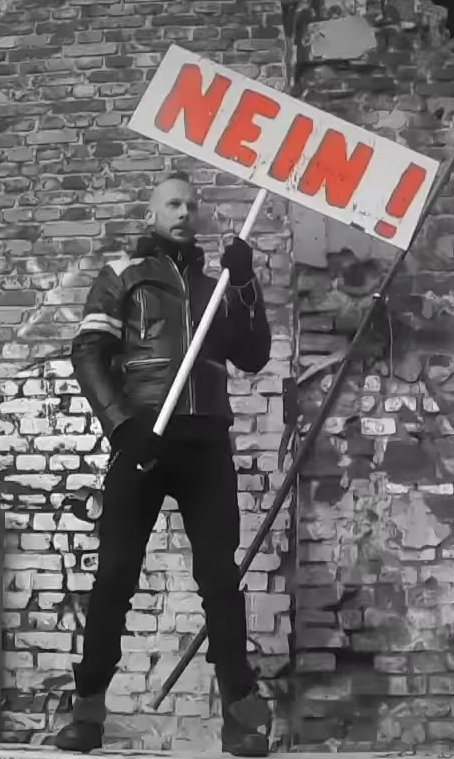
\includegraphics[width=0.35\textwidth,center]{nein.png}
        \hspace*{6cm}
        \href{https://www.youtube.com/watch?v=_dRra4786Ww}
             {\color{white}\fontsize{5pt}{0}\selectfont @Unzucht}

    }
    \end{center}
\end{frame}

\begin{frame}[fragile]{}
    \frametitle{}

    \begin{center}
        \begin{itemize}[label={\MVRightarrow}]
            \item Buffered (Lazy) B-Tree
            \item Cache conscious B-Tree
            \item Distributed B-Tree
            \item SB-Tree
            \item MDAM
            \item LSM Tree
            \item Trie
            \item ...
        \end{itemize}
    \end{center}
\end{frame}
\note{
    Buffered B-Tree are used in WiredTiger.
    Skip list are used also in WiredTiger as in memory structure, in Apache
    Cassandra again as in memory, and in Redis.
}

\begin{frame}[fragile]{}
    \frametitle{}

    \begin{center}
    \vspace{0.5cm}
    \includegraphics[width=0.4\textwidth,center]{internals.jpg}
    \end{center}
\end{frame}

\fontsize{18pt}{18}\selectfont
\begin{frame}
  \vspace*{2.5cm}
  \begin{minipage}[b][\paperheight]{\textwidth}
  \begin{center}

      %\raggedright%
      \linespread{1.0}%
      \usebeamerfont{title}%
      \usebeamercolor[fg]{title}%
      \if@noSmallCapitals%
        Questions?
      \else%
        \scshape{\color{black} Questions?}%
      \fi%
      \vspace*{0.3em}

      \usebeamerfont{subtitle}%
      \fontsize{13pt}{14}\selectfont
      \usebeamercolor[fg]{subtitle}%
        \begin{itemize}[label={}]
            \item {\color{black} \twitter\ @erthalion}
            \item {\color{black} \email\ ddolgov at redhat dot com}
        \end{itemize}
      \vspace*{2.5em}%

    \vfill
    \vspace*{2em}
  \end{center}
  \end{minipage}

\end{frame}
\note{
    ClickHouse - B-Tries
    HyPer - ART
    MSFT Hekaton - Bw-Tree
    Redis, MemSQL - Skip list
    Silo - Masstree
}

\end{document}
